\chapter{Resultados}
\label{chap:resultados}


\drop{A} lo largo de este capítulo, se desarrolla los resultados obtenidos según la evolución en cada uno de los aspectos de la plataforma de juego.
\begin{itemize}
\item Estructura de la aplicación.
\item Comunicaciones cliente-servidor.
\item Sistema de localización.
\item Lectura, tratamiento y comunicación de datos, de los sensores.
\item Gestión de eventos de la aplicación. Máquina de estados.
\item Diseño software de la interfaz gráfica.
\item Actualización software de la aplicación.
\end{itemize}


\section{Estructura de la aplicación.}
El funcionamiento de los dispositivos \emph{TUIO1} y \emph{TUIO1} es gestionado con el uso de \emph{Maquinas de Estado Finitos (FSM)}\footnote{Finite State Machine.}.


\subsection{Máquina de estados finitos dispositivo TUIO1.}

\begin{itemize}
\item \textbf{IDLE:} Estado inicial del dispositivo \emph{TUIO1}. La máquina permanece en este estado hasta recibir confirmación de comunicación con el dispositivo \emph{TUIO2}.\\
\textbf{Transiciones/eventos.}
\begin{itemize}
\item \texttt{tuio2\_connect:} transición de estado \textbf{IDLE} a \textbf{MAIN} cuando se establece las comunicaciones cliente-servidor.
\item \texttt{exit\_tuio1:} transición de estado \textbf{IDLE} a \textbf{EXIT} al recibir el evento salir de la aplicación.
\item \texttt{init\_server:} evento interno para iniciar el servidor.
\end{itemize}


\item \textbf{MAIN:} Estado principal de la aplicación una vez establecida la comunicación entre los dispositivos \emph{TUIO1} y \emph{TUIO2}.\\
\textbf{Transiciones/eventos.}
\begin{itemize}
\item \texttt{tuio2\_disconnect:} transición desde el estado \textbf{MAIN} a \textbf{IDLE} cuando se han perdido las comunicaciones con \emph{TUIO2}.
\item \texttt{start\_game:} transición desde el estado \textbf{MAIN} a \textbf{GAME}, al recibir el evento de comenzar el juego.
\item \texttt{exit\_tuio1:} transición de estado \textbf{IDLE} a \textbf{EXIT} al recibir el evento salir de la aplicación.
\end{itemize}


\item \textbf{GAME:} El dispositivo comienza a ejecutar el juego. Se crea un evento de salida para el dispositivo \emph{TUIO2}, el cual recibe la orden de cambiar su estado a \textbf{GAME}.\\
\textbf{Transiciones/eventos.}
\begin{itemize}
\item \texttt{stop\_game:} transición desde el estado \textbf{GAME} a \textbf{MAIN} al recibir el evento de finalizar el juego.
\item \texttt{tuio2\_disconnect:} transición desde el estado \textbf{GAME} a \textbf{IDLE} cuando se han perdido las comunicaciones con \emph{TUIO2}.
\item \texttt{exit\_tuio1:} transición de estado \textbf{GAME} a \textbf{EXIT} al recibir el evento salir de la aplicación.
\item \texttt{request\_data:} evento de salida para solicitar datos al dispositivo \emph{TUIO2}.
\item \texttt{receive\_data:} evento de entrada al recibir datos desde el dispositivo \emph{TUIO2}.
\end{itemize}


\item \textbf{EXIT:} Estado de la máquina por el cual se finaliza toda la aplicación.\\
\textbf{Eventos.}
\begin{itemize}
\item \texttt{exit\_tuio1:} evento de entrada para finalizar la ejecución de la aplicación.
\end{itemize}
\end{itemize}

La Figura ~\ref{fig:tuio1fsmv0} muestra la estructura de la máquina de estados del dispositivo \emph{TUIO1}

\begin{figure}[!h]
\begin{center}
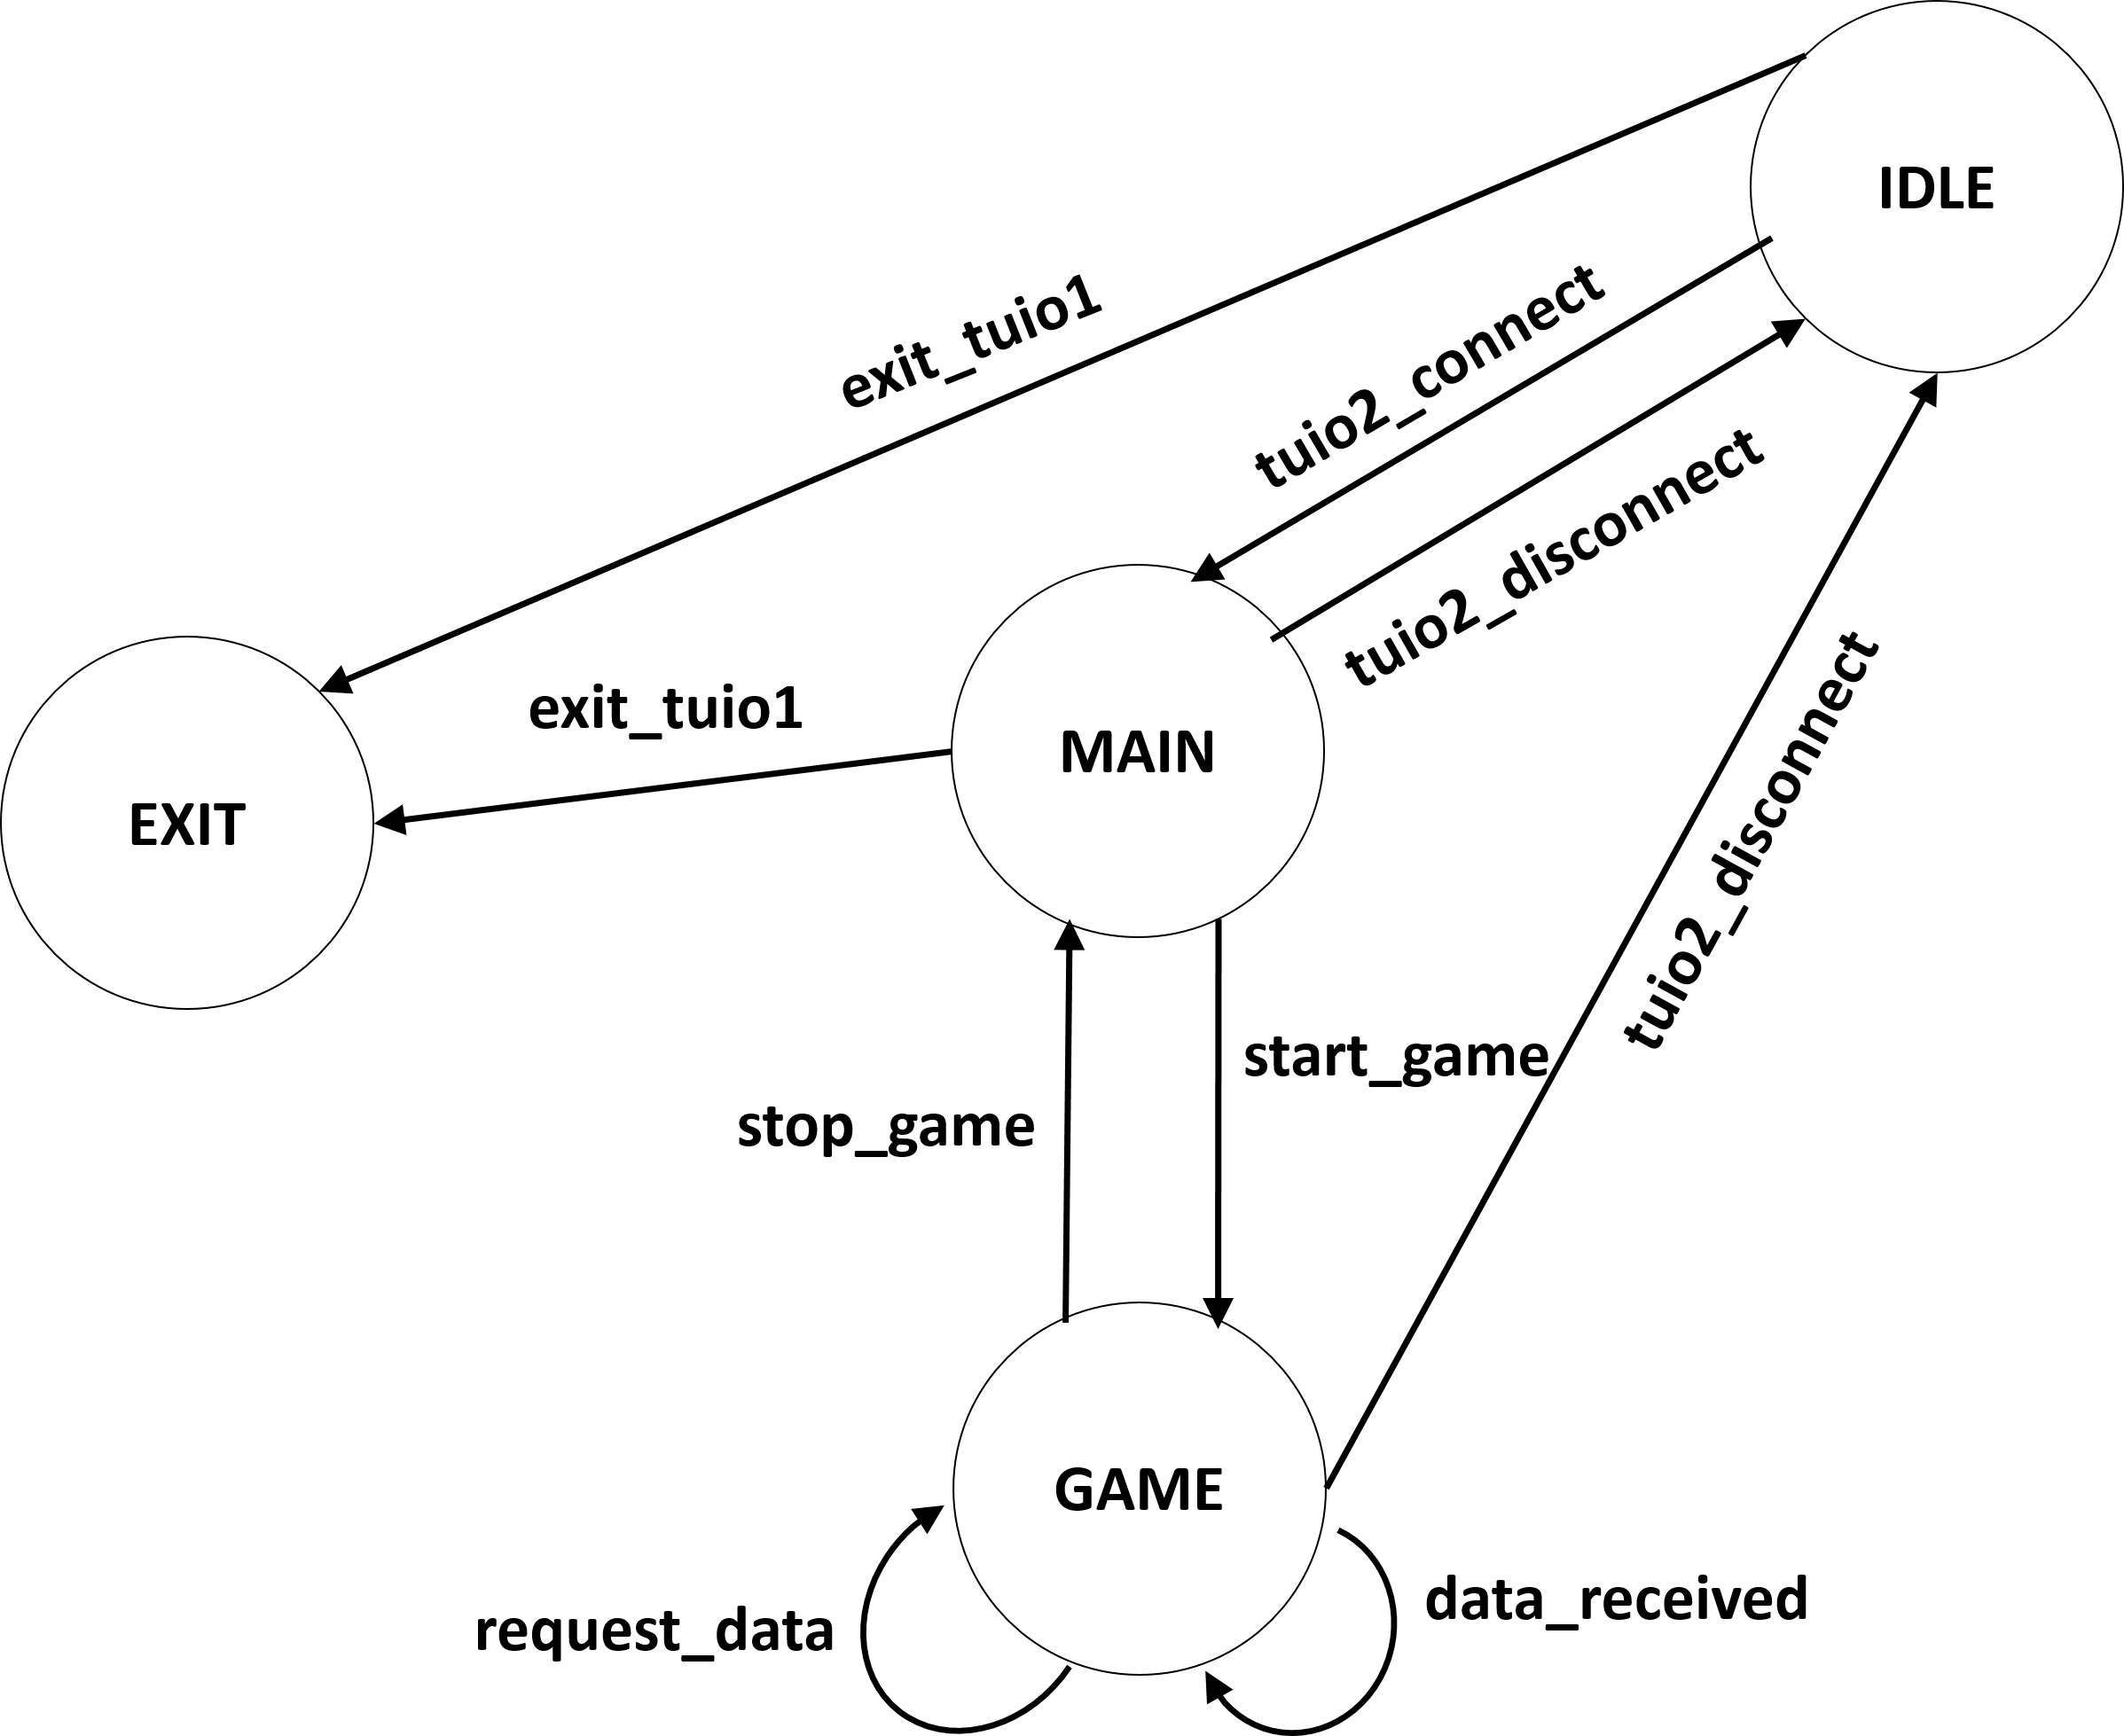
\includegraphics[width=0.7\textwidth]{fsm_tuio1_v0.png}
\caption{Estructura máquina de estados finitos TUIO1 (versión pruebas).}
\label{fig:tuio1fsmv0}
\end{center}
\end{figure}



\subsection{Máquina de estados finitos Servidor.}

\begin{itemize}
\item \textbf{IDLE:} Estado inicial del servidor a la espera de recibir un evento desde la máquina de estados del dispositivo \emph{TUIO1} para iniciar el servidor. Dispone de dos transiciones de estado posible, y tres eventos de entrada.\\
\textbf{Transiciones/Eventos.}
\begin{itemize}
\item \texttt{init\_server:} transición al estado \textbf{LISTEN}. La ejecución de esta transición sucede cuando la máquina de estados del servidor recibe el evento \texttt{init\_server} dentro de la máquina de estados \texttt{ServerFSM}. El evento puede ser creado por tres posibles entradas.
\item \texttt{close\_server:} transición al estado \textbf{EXIT} al recibir el evento \texttt{close\_server} desde la máquina de estados \texttt{Tuio1FSM}, para cerrar el servidor.\\
\item \texttt{create\_server}. Entrada desde la máquina de estados \texttt{Tuio1FSM}, al iniciar el dispositivo.
\item \texttt{reconnect}(perdida de conexión). Entrada de evento de reconexión al interrumpirse la conexión con el cliente \emph{(TUIO2)}.
\item \texttt{reconnect}(tiempo de espera). Agotado tiempo de espera para conectar con \emph{TUIO2}.
\end{itemize}


\item \textbf{LISTEN:} El servidor queda a la espera de conectar con el cliente (\emph{TUIO2}). En el caso de no conectar con el cliente (en un tiempo definido de 10 segundos), es ejecutada la transición \texttt{reconnect}. 
Al conectar con \emph{TUIO2} (cliente), \emph{ServerFSM} ejecuta la transición \texttt{wait\_data} hasta el estado \textbf{CONNECT}, a la espera de recibir datos desde \emph{TUIO2}. Al establecer la conexión con el cliente, se crea un evento de entrada indicando que las comunicaciones han sido establecidas.
\textbf{Transiciones.}
\begin{itemize}
\item \texttt{reconnect}: la máquina vuelve al estado \textbf{IDLE}, al agotarse el tiempo de espera para conectar con el cliente. Se crea el evento \emph{init\_server}, para volver a iniciar el servidor.\\
\item \texttt{close\_server:} transición al estado \textbf{EXIT} al recibir el evento \texttt{close\_server} desde la máquina de estados \texttt{Tuio1FSM}, para cerrar el servidor.\\
\textbf{Entradas.}
\item \texttt{init\_server:} el servidor queda a la espera de conectar con el cliente \emph{TUIO2}.
\end{itemize}


\item \textbf{CONNECT:} Existe comunicación entre los dispositivos \emph{TUIO1} y \emph{TUIO2}. 
Dispone de dos entradas y una transición posible: recibir datos, enviar datos, o volver a iniciar el servidor si la conexión ha sido interrumpida respectivamente.\\
\textbf{Transiciones.}
\begin{itemize}
\item \texttt{reconnect}: la máquina vuelve al estado \textbf{IDLE}, al interrumpirse la comunicación con el cliente. Se crea el evento \emph{init\_server}, para volver a iniciar el servidor.
\item \texttt{close\_server:} transición al estado \textbf{EXIT} al recibir el evento \texttt{close\_server} desde la máquina de estados \texttt{Tuio1FSM}, para cerrar el servidor.\\
\textbf{Entradas.}
\item \texttt{receive\_data} es ejecutada si se reciben datos desde \emph{TUIO2}. Los datos son añadidos a una lista (cola), la cual es manejada por \emph{Tuio1FSM} (por medio de \texttt{data\_received}). Se mantiene en el estado \textbf{CONNECT}, a la espera de recibir mas datos desde \emph{TUIO2}.
\item \texttt{send\_data:} envia datos al cliente \texttt{TUIO2}.
\end{itemize}


\item \textbf{EXIT:} Estado de la máquina por el cual se finaliza el servidor.\\
\textbf{Eventos.}
\begin{itemize}
\item \texttt{close\_server:} evento de entrada para finalizar la ejecución del servidor.
\end{itemize}
\end{itemize}

La Figura ~\ref{fig:fsmserverv0} muestra la estructura de la máquina de estados del dispositivo \emph{TUIO2}

\begin{figure}[!h]
\begin{center}
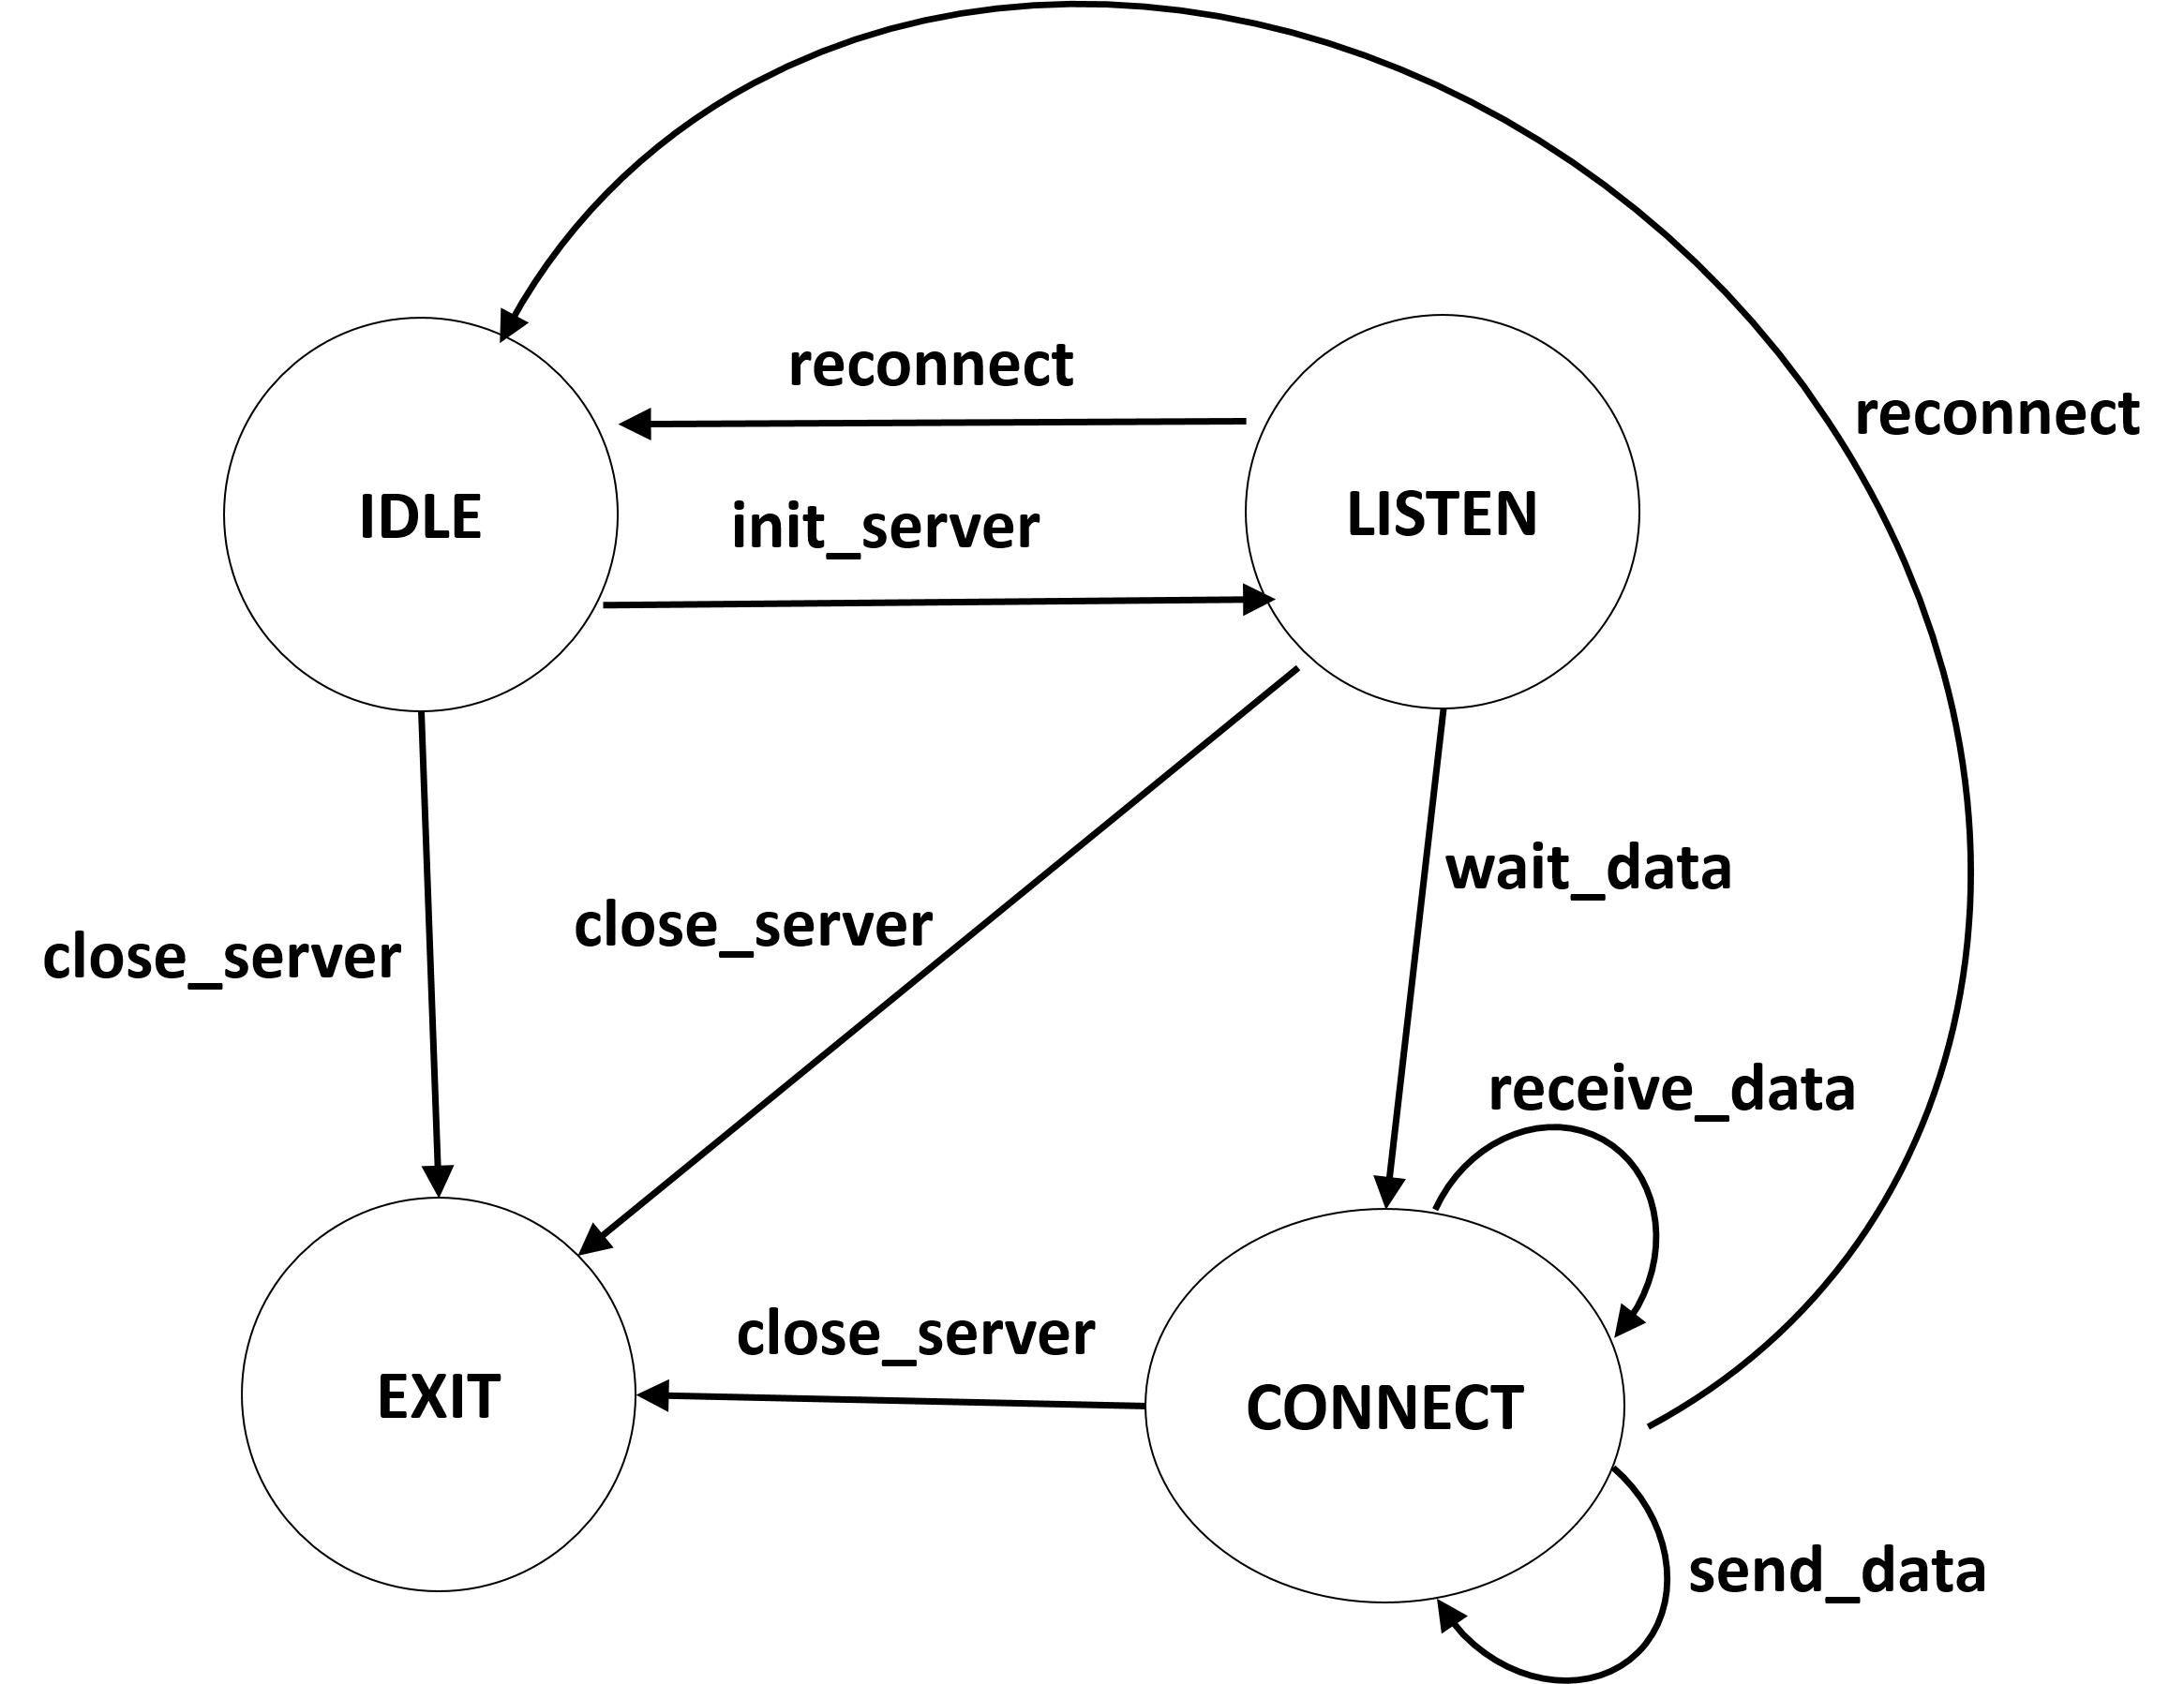
\includegraphics[width=0.7\textwidth]{fsm_server_v0.png}
\caption{Estructura máquina de estados finitos del servidor (versión pruebas).}
\label{fig:fsmserverv0}
\end{center}
\end{figure}




\subsection{Máquina de estados finitos dispositivo TUIO2.}

\begin{itemize}
\item \textbf{IDLE:} Estado inicial del dispositivo \emph{TUIO2}. La máquina permanece en este estado hasta recibir confirmación de comunicación con el dispositivo \emph{TUIO1}.\\
\textbf{Transiciones/eventos.}
\begin{itemize}
\item \texttt{tuio1\_connect:} transición de estado \textbf{IDLE} a \textbf{MAIN} cuando se establece las comunicaciones cliente-servidor.
\item \texttt{exit\_tuio2:} transición de estado \textbf{IDLE} a \textbf{EXIT} al recibir el evento salir de la aplicación.
\item \texttt{init\_client:} evento interno para iniciar el cliente.
\end{itemize}


\item \textbf{MAIN:} Estado principal de la aplicación una vez establecida la comunicación entre los dispositivos \emph{TUIO1} y \emph{TUIO2}.\\
\textbf{Transiciones/eventos.}
\begin{itemize}
\item \texttt{tuio1\_disconnect:} transición desde el estado \textbf{MAIN} a \textbf{IDLE} cuando se han perdido las comunicaciones con \emph{TUIO1}.
\item \texttt{start\_game:} transición desde el estado \textbf{MAIN} a \textbf{GAME}, al recibir el evento de comenzar el juego.
\item \texttt{exit\_tuio2:} transición de estado \textbf{IDLE} a \textbf{EXIT} al recibir el evento salir de la aplicación.
\end{itemize}


\item \textbf{GAME:} El dispositivo comienza a ejecutar el juego al recibir un evento desde el dispositivo \emph{TUIO1}, el cual envía la orden de cambiar el estado a \textbf{GAME}.\\
\textbf{Transiciones/eventos.}
\begin{itemize}
\item \texttt{stop\_game}: transición desde el estado \textbf{GAME} a \textbf{MAIN} al recibir el evento de finalizar el juego.
\item \texttt{tuio1\_disconnect}: transición desde el estado \textbf{GAME} a \textbf{IDLE} cuando se han perdido las comunicaciones con \emph{TUIO1}.
\item \texttt{exit\_tuio2:} transición de estado \textbf{GAME} a \textbf{EXIT} al recibir el evento salir de la aplicación.
\item \texttt{send\_data}: evento de salida para enviar datos al dispositivo \emph{TUIO1}.
\item \texttt{data\_treatment}: evento de entrada para tratar datos/eventos recibidos desde el dispositivo \emph{TUIO1}.
\end{itemize}


\item \textbf{EXIT:} Estado de la máquina por el cual se finaliza toda la aplicación.\\
\textbf{Eventos.}
\begin{itemize}
\item \texttt{exit\_tuio2:} evento de entrada para finalizar la ejecución de la aplicación.
\end{itemize}
\end{itemize}

La Figura ~\ref{fig:tuio2fsmv0} muestra la estructura de la máquina de estados del dispositivo \emph{TUIO2}

\begin{figure}[!h]
\begin{center}
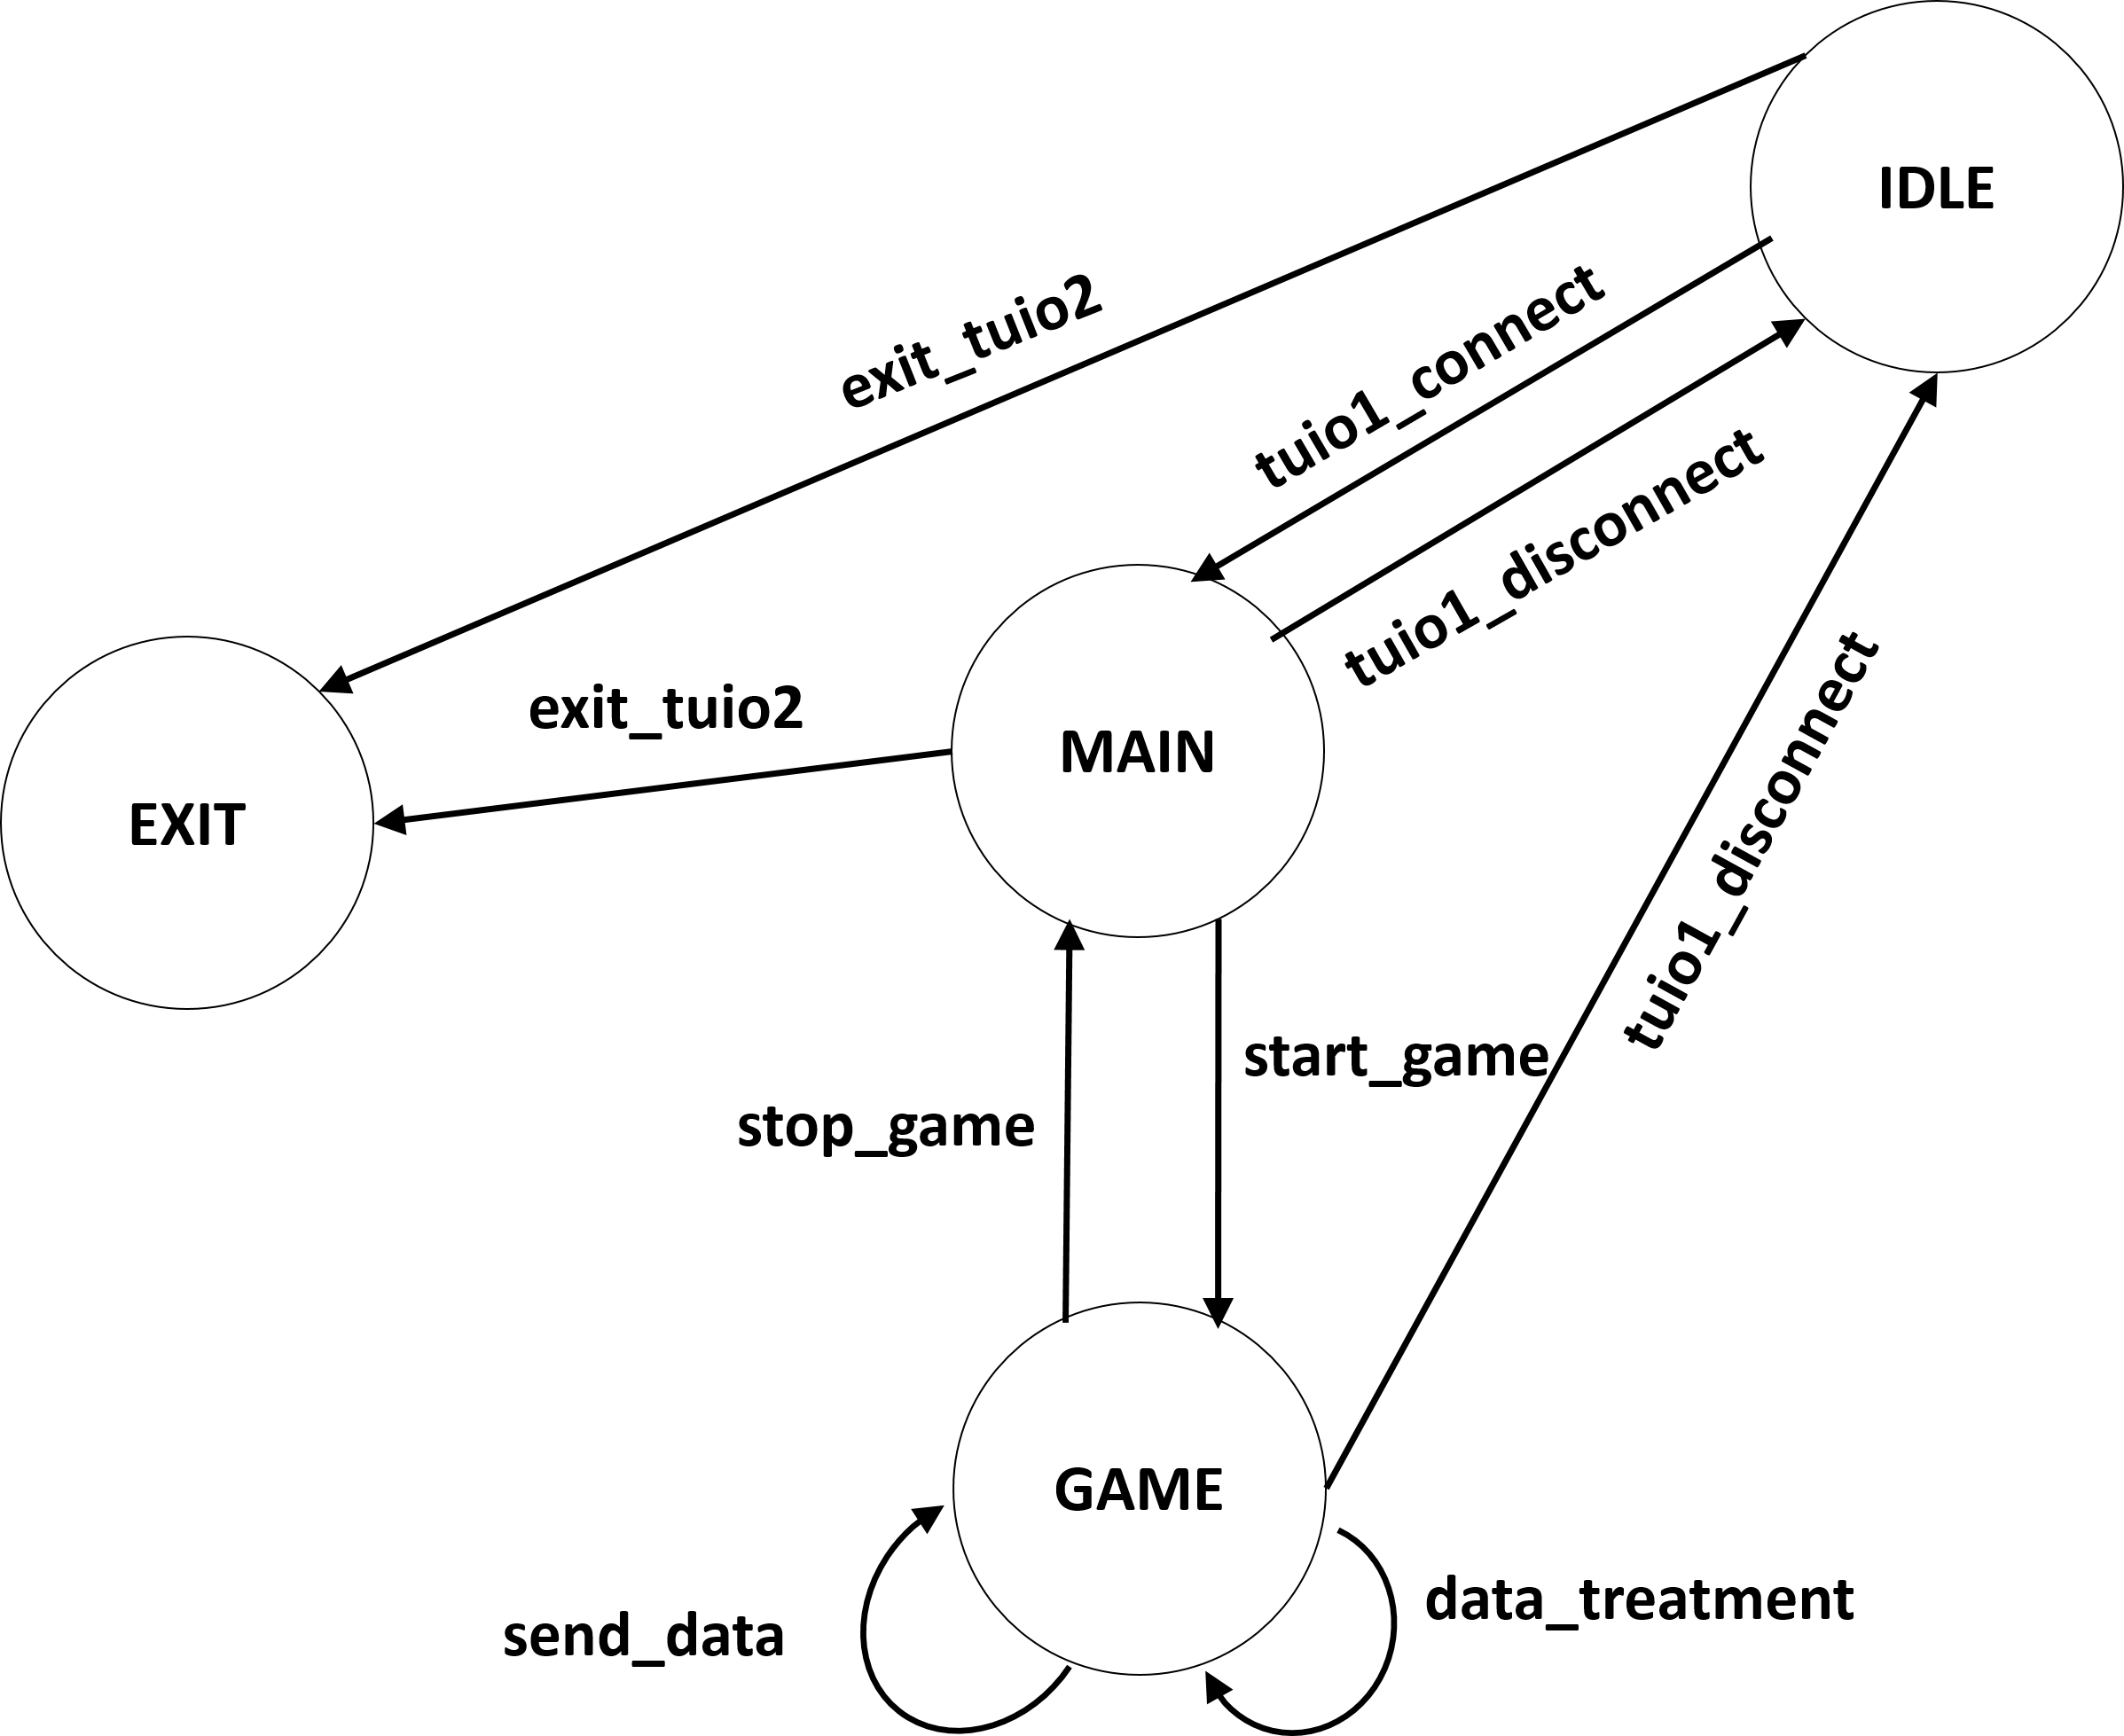
\includegraphics[width=0.7\textwidth]{fsm_tuio2_v0.png}
\caption{Estructura máquina de estados finitos TUIO2 (versión pruebas).}
\label{fig:tuio2fsmv0}
\end{center}
\end{figure}


\subsection{Máquina estados finitos Cliente.}

\begin{itemize}
\item \textbf{IDLE:} Estado inicial del cliente a la espera de recibir un evento desde la máquina de estados del dispositivo \emph{TUIO2} para iniciar el cliente. Dispone de dos transiciones de estado posible, y tres eventos de entrada.\\
\textbf{Transiciones/Eventos.}
\begin{itemize}
\item \texttt{init\_cliente:} transición al estado \textbf{LISTEN}. La ejecución de esta transición sucede cuando la máquina de estados del cliente recibe el evento \texttt{init\_cliente} dentro de la máquina de estados \texttt{ClientFSM}. El evento puede ser creado por tres posibles entradas.
\item \texttt{close\_client:} transición al estado \textbf{EXIT} al recibir el evento \texttt{close\_cliente} desde la máquina de estados \texttt{Tuio2FSM}, para cerrar el cliente.\\
\item \texttt{create\_client}. Entrada desde la máquina de estados \texttt{Tuio2FSM}, al iniciar el dispositivo.
\item \texttt{reconnect}(perdida de conexión). Entrada de evento de reconexión al interrumpirse la conexión con el servidor \emph{(TUIO1)}.
\item \texttt{reconnect}(tiempo de espera). Agotado tiempo de espera para conectar con \emph{TUIO1}.
\end{itemize}


\item \textbf{LISTEN:} El servidor queda a la espera de conectar con el servidor (\emph{TUIO1}). En el caso de no conectar con el servidor (en un tiempo definido de 10 segundos), es ejecutada la transición \texttt{reconnect}. 
Al conectar con \emph{TUIO1} (servidor), \emph{ClientFSM} ejecuta la transición \texttt{wait\_data} hasta el estado \textbf{CONNECT}, a la espera de recibir datos desde \emph{TUIO1}. Al establecer la conexión con el servidor, se crea un evento de entrada indicando que las comunicaciones han sido establecidas.
\textbf{Transiciones.}
\begin{itemize}
\item \texttt{reconnect}: la máquina vuelve al estado \textbf{IDLE}, al agotarse el tiempo de espera para conectar con el servidor. Se crea el evento \emph{init\_client}, para volver reestablecer el cliente.\\
\item \texttt{close\_client:} transición al estado \textbf{EXIT} al recibir el evento \texttt{close\_client} desde la máquina de estados \texttt{Tuio2FSM}, para cerrar el cliente.\\
\textbf{Entradas.}
\item \texttt{init\_client:} el cliente queda a la espera de conectar con el servidor \emph{TUIO1}.
\end{itemize}


\item \textbf{CONNECT:} Existe comunicación entre los dispositivos \emph{TUIO1} y \emph{TUIO2}. 
Dispone de dos entradas y una transición posible: recibir datos, enviar datos, o volver a iniciar el cliente si la conexión ha sido interrumpida respectivamente.\\
\textbf{Transiciones.}
\begin{itemize}
\item \texttt{reconnect}: la máquina vuelve al estado \textbf{IDLE}, al interrumpirse la comunicación con el servidor. Se crea el evento \emph{init\_client}, para volver a iniciar el cliente.
\item \texttt{close\_client:} transición al estado \textbf{EXIT} al recibir el evento \texttt{close\_client} desde la máquina de estados \texttt{Tuio2FSM}, para cerrar el cliente.\\
\textbf{Entradas.}
\item \texttt{receive\_data} es ejecutada si se reciben datos desde \emph{TUIO1}. Los datos son añadidos a una lista (cola), la cual es manejada por \emph{Tuio2FSM} (por medio de \texttt{data\_treatment
}). Se mantiene en el estado \textbf{CONNECT}, a la espera de recibir mas datos desde \emph{TUIO1}.
\item \texttt{send\_data:} envía datos al servidor \texttt{TUIO1}.
\end{itemize}


\item \textbf{EXIT:} Estado de la máquina por el cual se finaliza el cliente.\\
\textbf{Eventos.}
\begin{itemize}
\item \texttt{close\_client:} evento de entrada para finalizar la ejecución del cliente.
\end{itemize}
\end{itemize}

La Figura ~\ref{fig:fsmclientv0} muestra la estructura de la máquina de estados del cliente.

\begin{figure}[!h]
\begin{center}
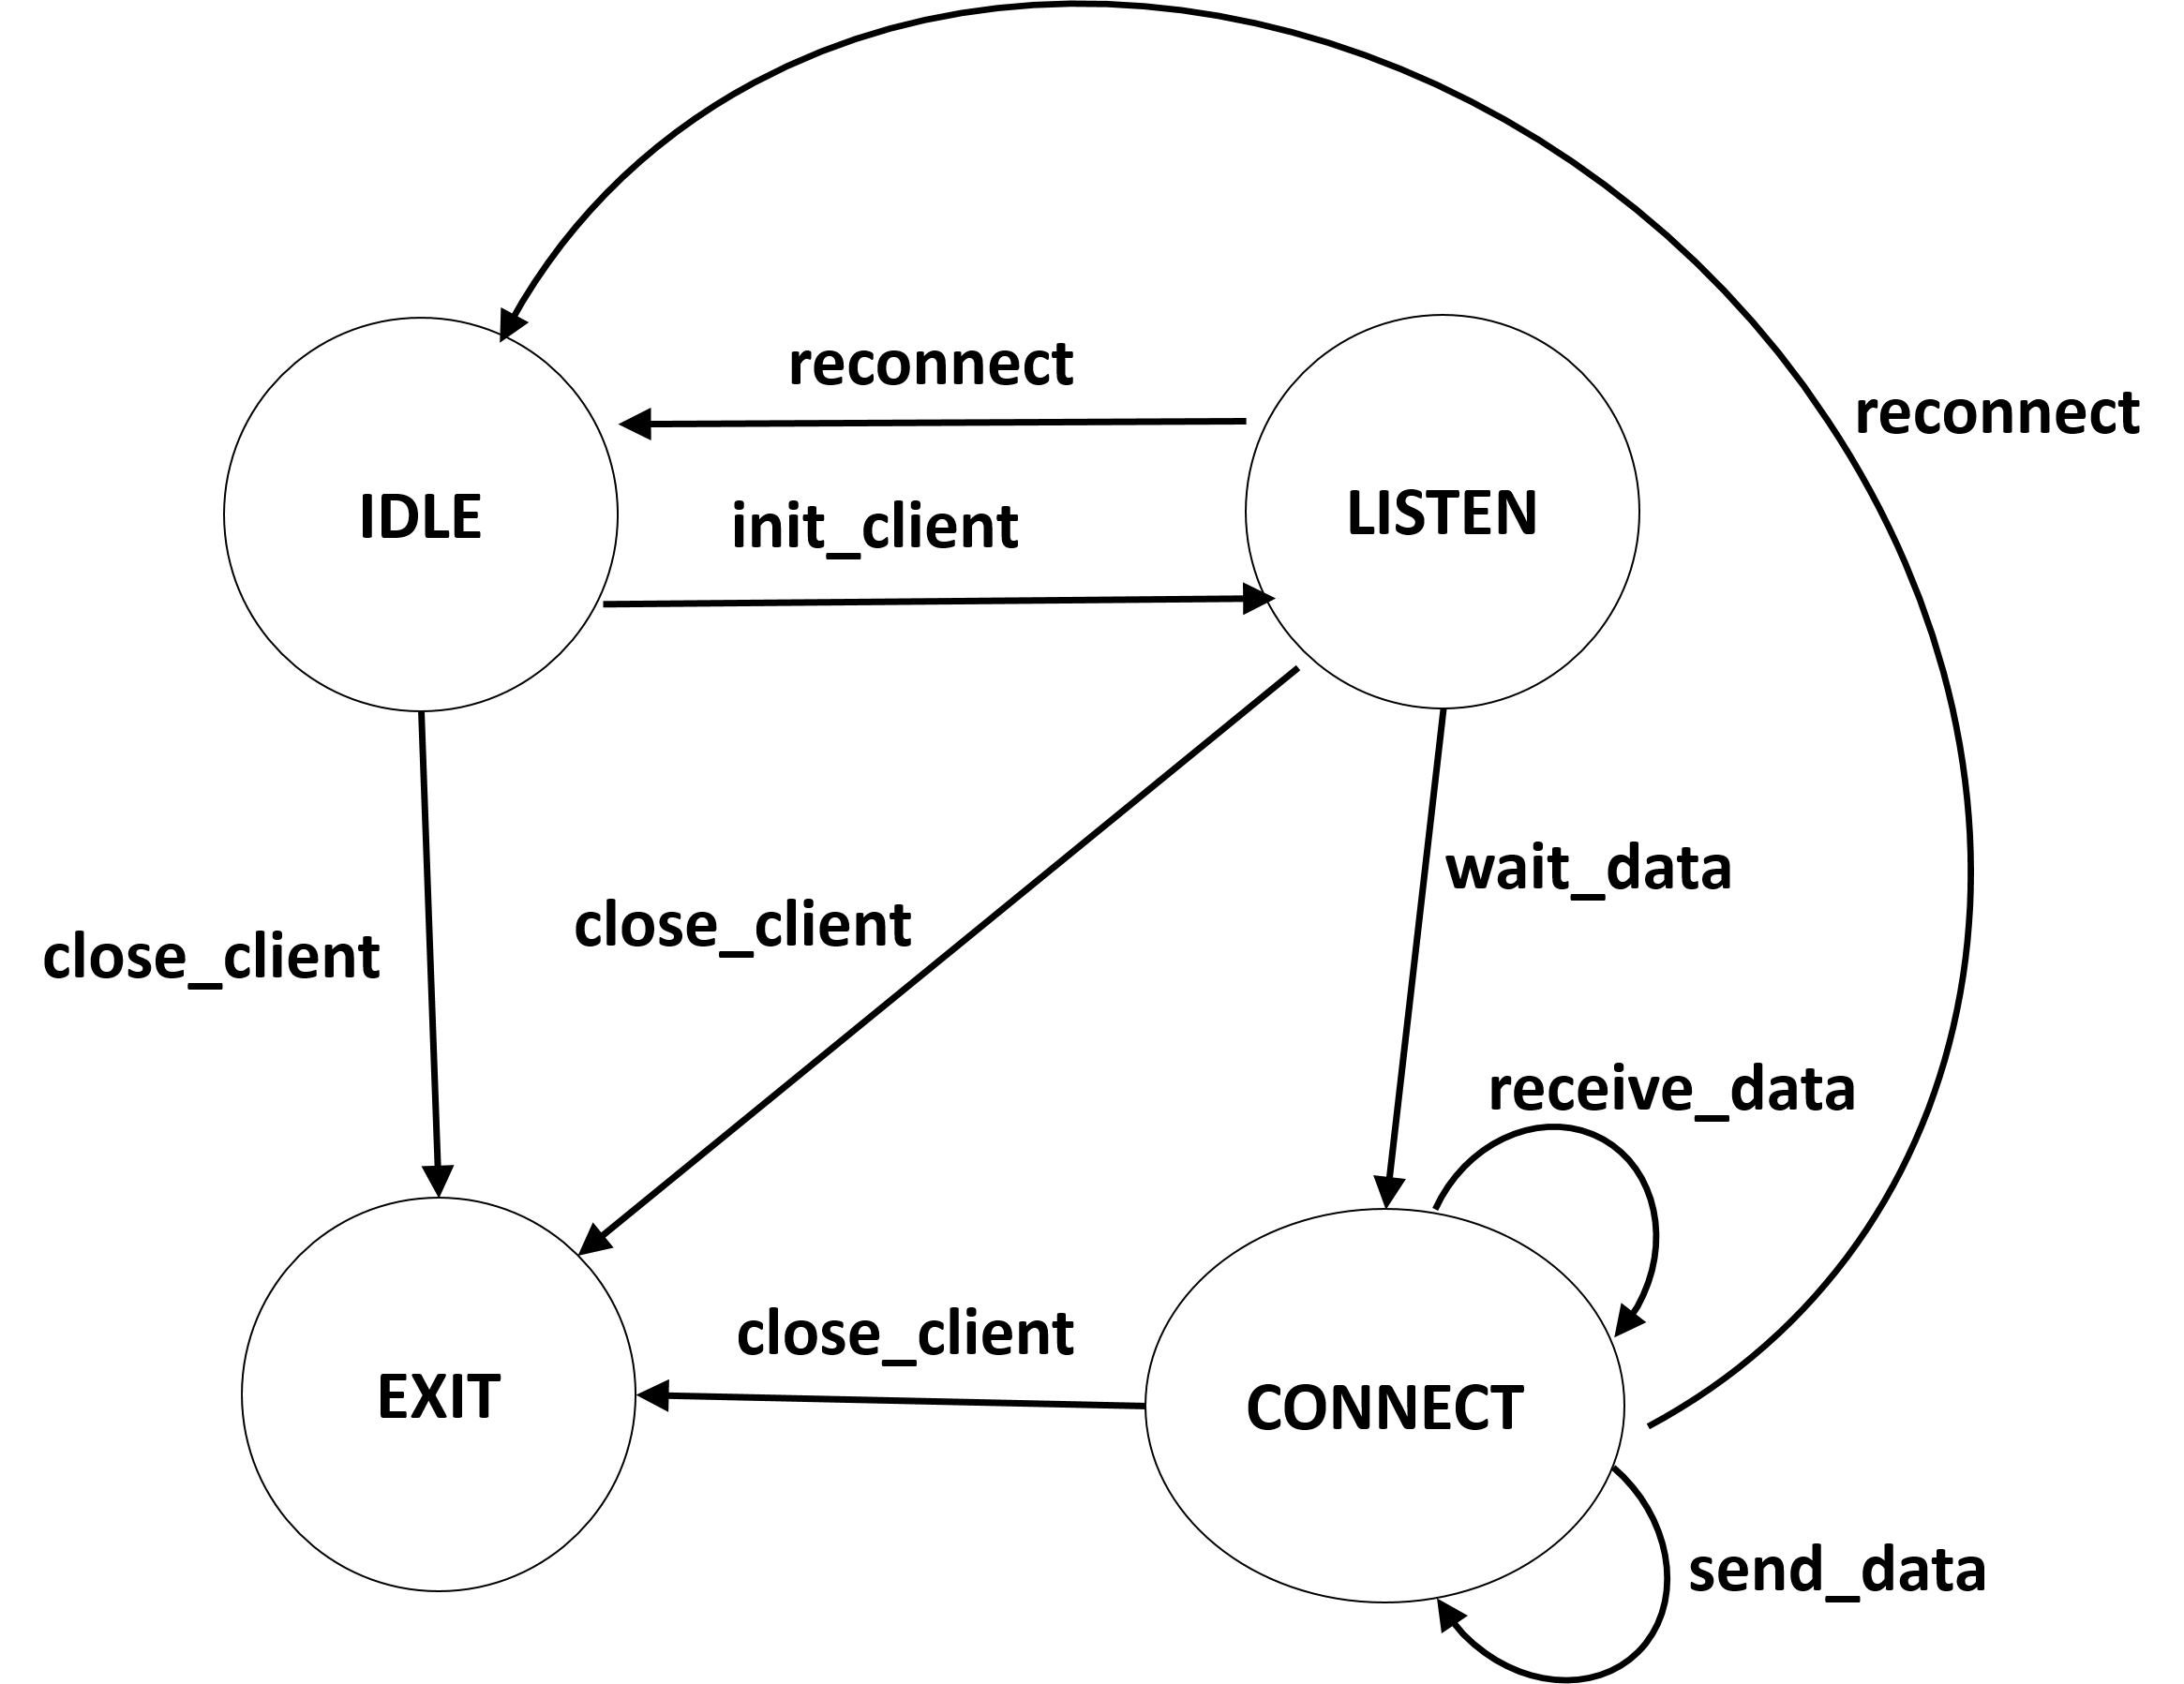
\includegraphics[width=0.7\textwidth]{fsm_client_v0.png}
\caption{Estructura máquina de estados finitos del cliente (versión pruebas).}
\label{fig:fsmclientv0}
\end{center}
\end{figure}

\section{Comunicaciones cliente-servidor.}
\label{sec:comunicaciones}
Siguiendo la estructura expuesta en la sección anterior, se escribe el código para crear las máquinas de estados finitos para ambos dispositivos.

Disposición de los archivos del dispositivo \emph{TUIO1:}
\begin{itemize}
\item Código principal y máquina de estados de la aplicación: \texttt{\textbackslash itanium\textbackslash Tuio1.py}
\item Código y máquina de estados del servidor: \texttt{\textbackslash itanium\textbackslash lib\textbackslash Server.py}
\end{itemize} 

Disposición de los archivos del dispositivo \emph{TUIO2:}
\begin{itemize}
\item Código principal y máquina de estados de la aplicación: \texttt{\textbackslash itanium\textbackslash Tuio2.py}
\item Código y máquina de estados del cliente: \texttt{\textbackslash itanium\textbackslash lib\textbackslash Client.py}
\item Código y máquina de estados del sensor \emph{MPU-9255}: \texttt{\textbackslash itanium\textbackslash lib\textbackslash MPU9255.py}
\end{itemize}

\subsection{Programa de pruebas de las comunicaciones cliente-servidor.}

El programa de pruebas consiste en realizar él envió/recepción de datos entre los dispositivos, donde se realizan secuencias básicas en las comunicaciones.
La secuencia que realiza el programa de pruebas en las comunicaciones cliente servidor, es la siguiente:

El servidor se inicia en el \emph{puerto 8888} y queda a la espera de la conexión del cliente. Se imprime por pantalla lado servidor: «Esperando cliente». 

Una vez el cliente establece la comunicación con el servidor, se imprime por pantalla en lado servidor: «Cliente conectado». De igual manera, en el lado cliente se imprime por pantalla: «Conectado a servidor».

Se crea un evento para indicar a ambos dispositivos que se inicie el juego (estado \textbf{GAME}). Se imprime por pantalla el mensaje: «Juego iniciado»

Cuando ambos dispositivos estén en el estado \textbf{GAME}, el servidor envía una petición de datos de la unidad de medición inercial \emph{MPU-9255}.

Este evento es gestionado en el programa principal \texttt{tuio2}, que devuelve la petición solicitada del servidor. Se imprime por pantalla: «Datos enviados al servidor.». Son mostrados los datos recibidos en el servidor, una vez manejado el evento de entrada: «Datos recibidos del cliente: » 

Finaliza la conexión y la aplicación de ambos dispositivos, mostrando respectivamente: «Aplicación finalizada»

La Figura ~\ref{fig:fsmexample} muestra de manera gráfica, la secuencia básica expuesta para las pruebas de las comunicaciones.

\begin{figure}[!h]
\begin{center}
\includegraphics[width=0.7\textwidth]{fsm_example.png}
\caption{Estructura de la secuencia de las pruebas cliente-servidor.}
\label{fig:fsmexample}
\end{center}
\end{figure}


\section{Sistema de localización.}
El sistema de localización consiste en obtener las coordenadas de posición y ángulo del \emph{Widget tangible TUIO2} al ser posicionado sobre la pantalla táctil capacitiva del dispositivo \emph{TUIO1}. Estos eventos táctiles siguen un patrón determinado, cuya información es procesada para una interacción gráfica y tangible entre dispositivos.
Son dos las interacciones posibles mediante el sistema de localización: incorporar información gráfica de \emph{TUIO2} a \emph{TUIO1}, o \emph{extraer} información desde \emph{TUIO1} a \emph{TUIO2}.

Para generar estos eventos táctiles, el dispositivo \emph{TUIO2} dispone de tres almohadillas conductoras que al tomar contacto con la pantalla capacitiva, se generan varios eventos táctiles simultáneos.

\subsection{Versión de pruebas 1. Localización de coordenadas con patrón de triángulo rectángulo escaleno.}  

Ejemplo de aplicación del sistema de localización. Antes de posicionar «TUIO2» sobre «TUIO1», las pantallas de ambos dispositivos muestran imágenes diferentes (ver Figura~\ref{fig:Localizacion1}).
\begin{figure}[!h]
\begin{center}
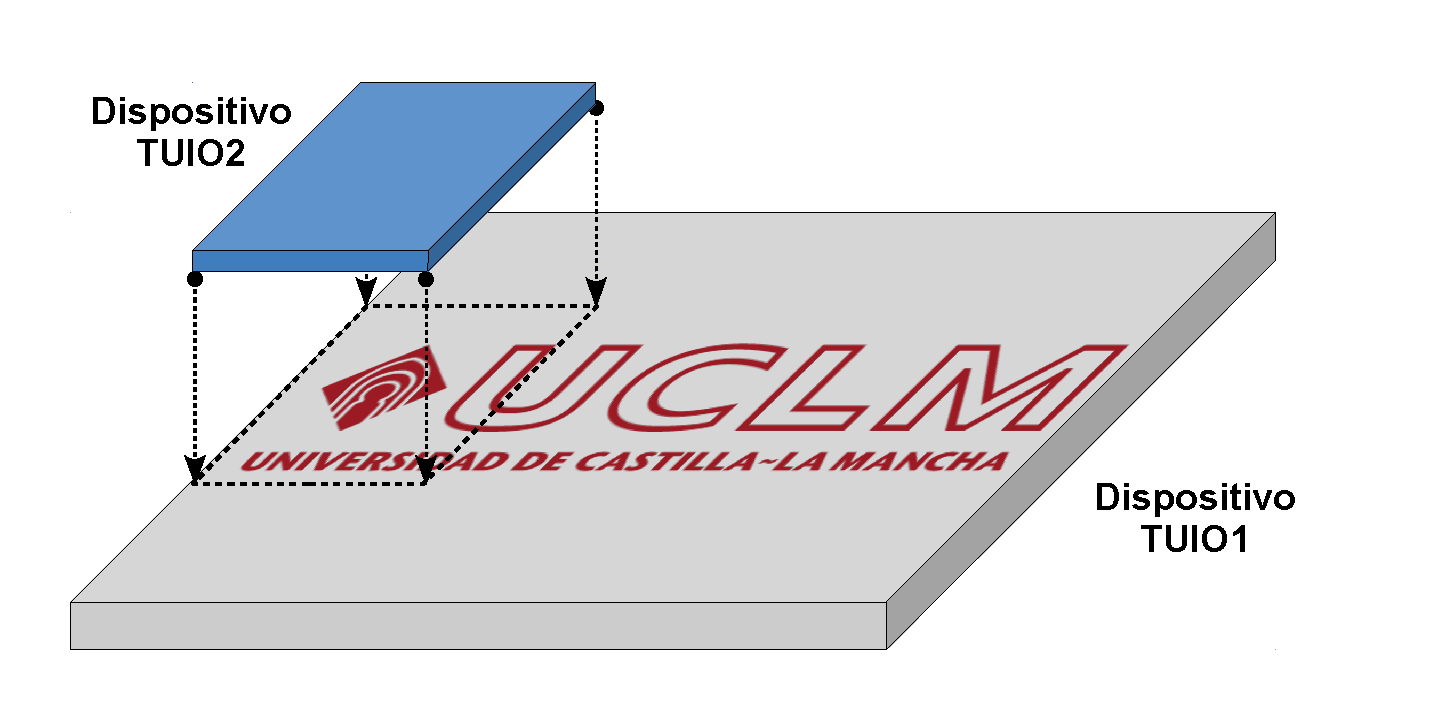
\includegraphics[width=0.7\textwidth]{localizacion1.pdf}
\caption{Posición de los dispositivos antes de la interacción sobre la pantalla capacitiva}
\label{fig:Localizacion1}
\end{center}
\end{figure}
Al posicionar \emph{TUIO2} sobre la pantalla de \emph{TUIO1}, la pantalla de \emph{TUIO2} muestra la parte de imagen correspondiente que es tapada por el dispositivo. (Figura~\ref{fig:Localizacion2}).
\begin{figure}[!h]
\begin{center}
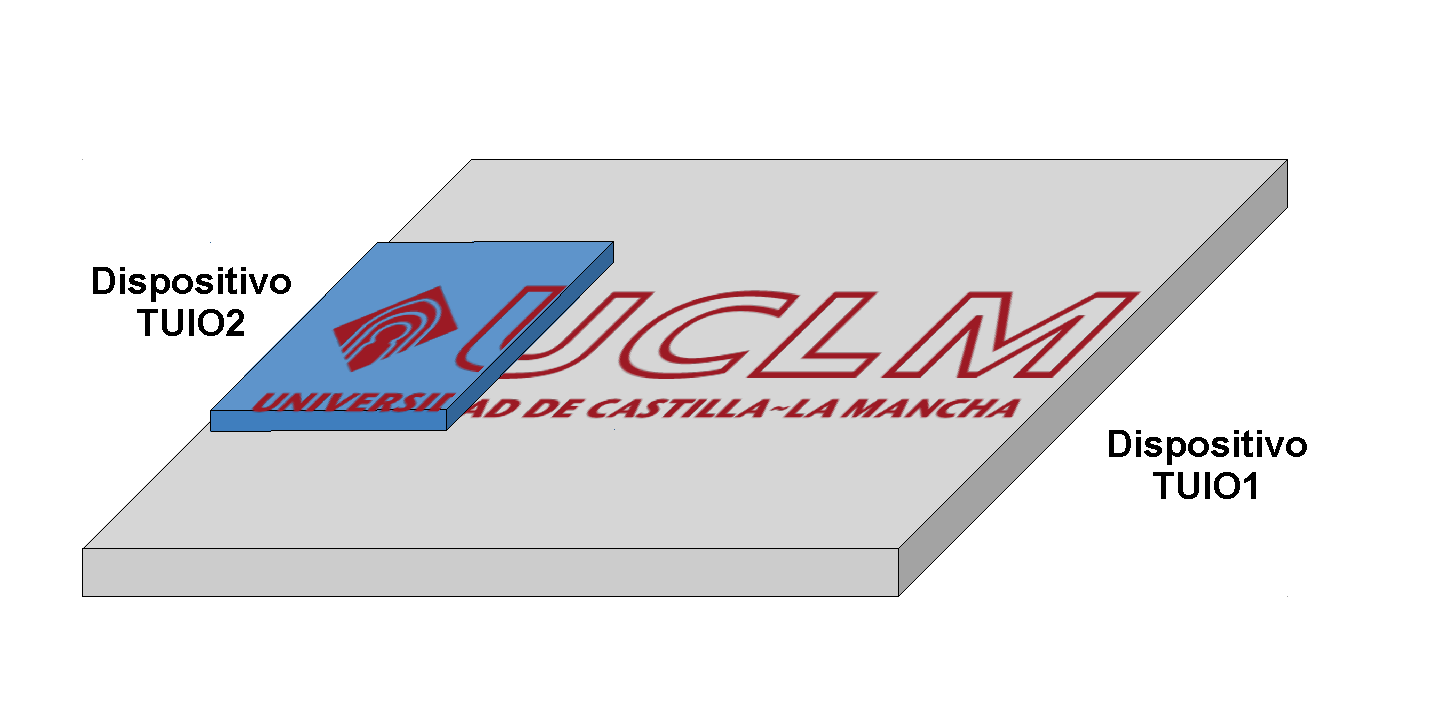
\includegraphics[width=0.7\textwidth]{localizacion2.pdf}
\caption{Posición de los dispositivos después de la interacción sobre la pantalla capacitiva}
\label{fig:Localizacion2}
\end{center}
\end{figure}

El procedimiento para obtener la posición se consigue con el uso del sensor capacitivo de la propia pantalla de \emph{TUIO1} que, al detectar una variación de la capacitancia, genera un evento táctil.
El dispositivo \emph{TUIO2} produce tres eventos táctiles sobre la pantalla capacitiva. Estos eventos son generados por medio de tres almohadillas de goma conductora, que están conectadas al borne negativo de la \emph{RaspberryPi}. Esta conexión evita que el usuario tenga que sostener con su propia mano el dispositivo, haciendo de conexión a tierra el propio borne negativo.
El diseño de los puntos de contacto es el que se muestra en la Figura~\ref{fig:Localizacion3}.
\begin{figure}[!h]
\begin{center}
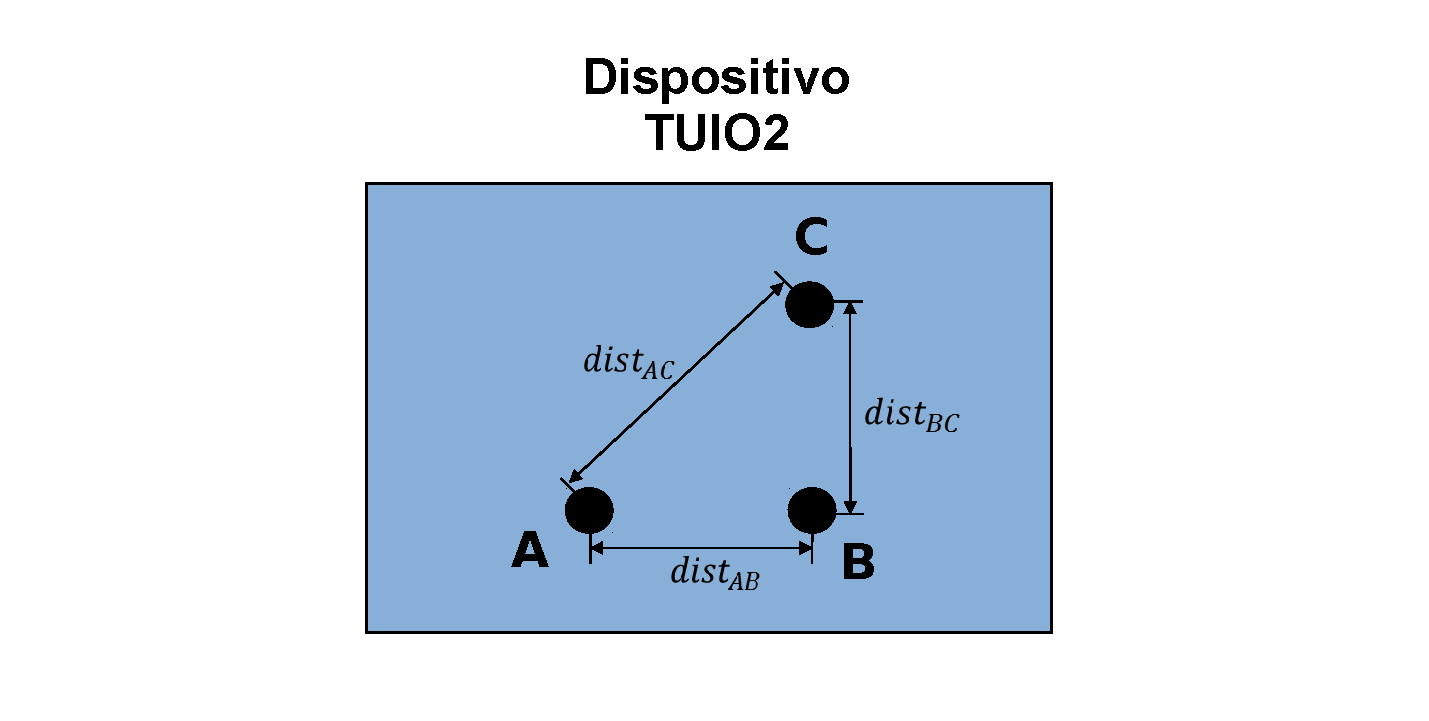
\includegraphics[width=0.9\textwidth]{localizacion3.pdf}
\caption{Disposición de las almohadillas conductoras en la parte inferior del \emph{widget tangible} para generar los eventos táctiles. }
\label{fig:Localizacion3}
\end{center}
\end{figure}
Los tres puntos de contacto son identificados con las letras \textbf{A, B} y \textbf{C}, que dan nombre a los vértices de un triángulo rectángulo escaleno que forman. Se ha elegido este tipo de diseño, ya que cada uno de los tres lados tiene una medida diferente, lo que hace que sea más fácil identificar cada segmento del triángulo, y así evitar posibles problemas cuando se localice cualquiera de sus vértices.

Cuando \emph{TUIO2} está sobre la pantalla, los eventos táctiles generados, proporcionan la siguiente información al dispositivo \emph{TUIO1}: posición de las coordenadas (x,y), y número de evento. Las coordenadas de la posición de cada evento táctil está expresada en \emph{pixels}, por lo que cada evento producido será manejado en esas unidades de media (ver Figura~\ref{fig:Localizacion4}).\\
\begin{figure}[!h]
\begin{center}
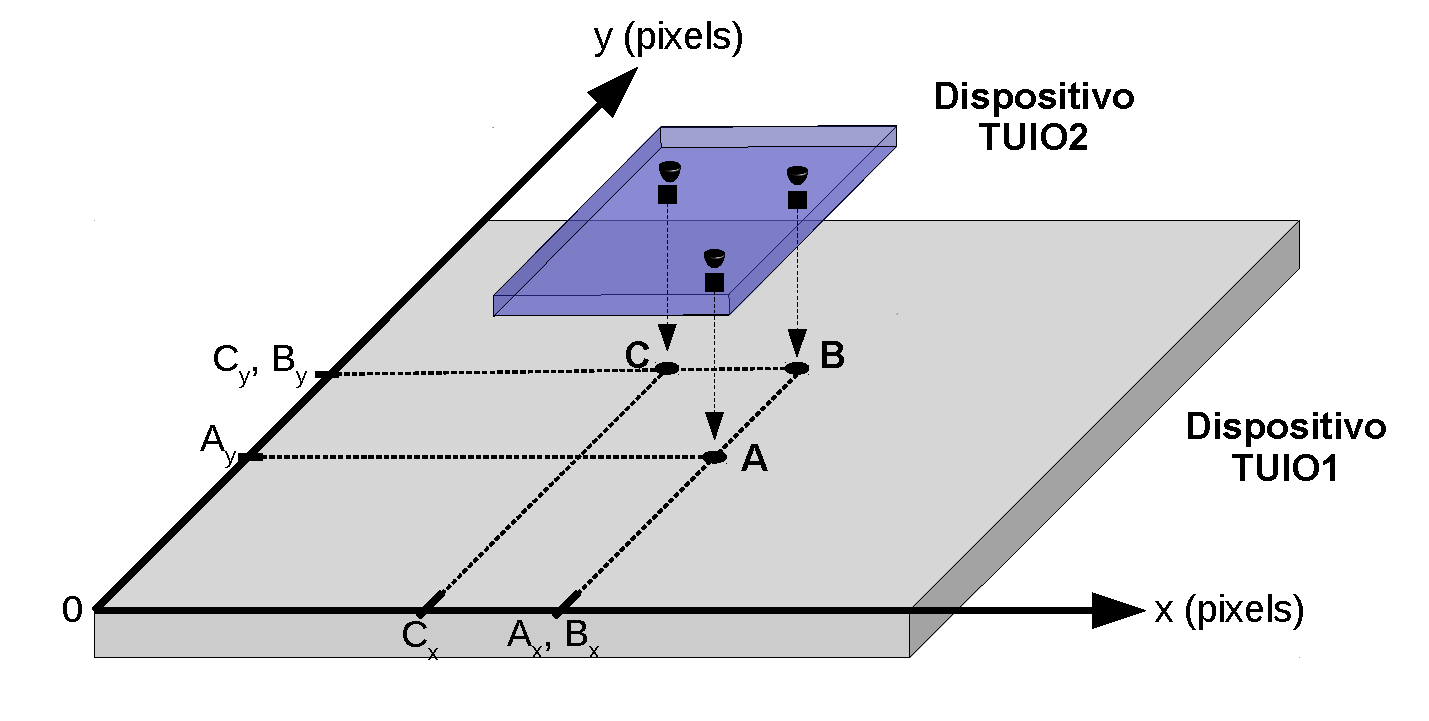
\includegraphics[width=0.9\textwidth]{localizacion4.pdf}
\caption{Coordenadas de los puntos \textbf{A, B} y \textbf{C} del \emph{widget tangible} sobre la pantalla capacitiva. }
\label{fig:Localizacion4}
\end{center}
\end{figure}
Estos datos son interpretados y tratados para calcular la posición de \emph{TUIO2} en una librería desarrollada en \emph{Python}.

\subsubsection{Librería para la localización.}

Todos los eventos táctiles generados sobre la pantalla capacitiva del dispositivo \emph{TUIO1} son manejados por la \emph{clase Widget} en \emph{Python}, con el método \texttt{on\_touch\_down().}\\
Este método obtiene la información de posición e ID del evento táctil producido, almacenando estos datos en la lista \texttt{touch[].}\\
Se crea una librería específica para el manejo de esta lista, la cual tratará y manejara los datos para obtener la información de posición de \emph{TUIO2}.

\textbf{Método \texttt{pulsacion(touch)}}\\
El argumento de entrada que corresponde con las coordenadas y número de evento táctil que contiene la lista de eventos (\texttt{touch}).\\
Estos datos son almacenados en la última posición de la lista \texttt{puls[]}aplicando el método \texttt{append()}:\\
\texttt{self.puls.append((t.x,t.y,t.id))}.\\
donde: \\
\texttt{t.x}: coordenada x del evento táctil.\\
\texttt{t.y}: coordenada y del evento táctil.\\
\texttt{t.id}: identificación del evento táctil (número de evento).\\
Cuando el número de eventos almacenados en \texttt{puls[]} 
es mayor que 1, se llama al método \texttt{determinar\_distancias()}.

\textbf{Método \texttt{determinar\_distancias()}}.\\
El método \texttt{Vector()}, de la librería \texttt{kivy}, calcula la distancia entre los eventos táctiles producidos hasta el momento, que son almacenados en la lista \texttt{puls[]}, recorriendo desde el último elemento de la lista \texttt{puls[]} hasta el primero. El método \texttt{determinar\_lados} determina las distancias entre puntos. Si la distancia es correcta, se incrementa la variable \texttt{contador}, la cual al llegar a 2, llama al método \texttt{determinar\_puntos()}.

\textbf{Método \texttt{determinar\_lados()}}.\\
Método para verificar si dos eventos táctiles de los cuales se ha determinado la distancia, corresponden con uno de los lados del triángulo del \emph{widget tangible}, donde \textit{m} corresponde con la distancia entre los dos eventos táctiles, \textit{i} el tamaño de la lista \texttt{puls[]}, y \textit{a} el número de iteración del bucle que recorre cada uno de los elementos de la lista \texttt{puls[]}.

Este método es llamado cada vez que el método \texttt{determinar\_distancias()} es invocado.
Se comprueba si la distancia entre los dos puntos corresponde con el rango de medidas establecidas para los lados del triángulo del \emph{widget tangible}. Los rangos de medida se muestran en la siguiente tabla (~\ref{tab:intervalos-coordenadas}).

\begin{table}[hp]
\centering
{\small



\begin{tabular}{p{.2\textwidth}p{.2\textwidth}}
  \tabheadformat
  \tabhead{Rango}   &
  \tabhead{Segmento del triángulo}  \\
\hline
(120,150) & AB \\
\hline
(160,150) & BC \\
\hline
(210,260) & AC
\end{tabular}


% Local variables:
%   coding: utf-8
%   ispell-local-dictionary: "castellano8"
%   TeX-master: "main.tex"
% End:

}
\caption[Intervalos de medida de cada segmento del triángulo]
{Intervalos de medida de cada segmento del triángulo}
\label{tab:intervalos-coordenadas}
\end{table}
Si la medida corresponde con alguno de los rangos establecidos, dicha medida es almacenada junto con las coordenadas de ambos eventos en la lista \texttt{dist[]}. Por ejemplo, si la distancia entre los dos eventos táctiles es correcta, y corresponde al segmento AB, los datos en la lista \texttt{dist[]} son almacenados de la siguiente manera:\\
\texttt{self.dist.append((m,'AB',toq1,toq2)) }\\
donde \texttt{m} corresponde a la distancia entre ambos puntos, \texttt{AB} es el nombre del segmento al que corresponde, \texttt{toq1} son las coordenadas del evento táctil con el cual se está midiendo la distancia en el método \texttt{determinar\_distancias()}, y \texttt{toq2} son las coordenadas del ultimo evento táctil.
Si la distancia es correcta se incrementa en una unidad la variable \texttt{contador}.

\textbf{Método \texttt{determinar\_puntos()}}.\\
Este método es invocado dentro del método \texttt{determinar\_distancias()} cuando la variable \texttt{contador} es mayor a 1, es decir, existen dos segmentos correctos del triángulo cuyos datos han sido almacenados en la lista \texttt{dist[]}, la cual contiene en ese momento dos elementos.
Los puntos del triángulo \textbf{(A,B,C)}, son calculados siguiendo la siguiente lógica:
Si los segmentos de los elementos de \texttt{dist[]} corresponden con $\overline{BC}$ y $\overline{AB}$ respectivamente, se llama al método \texttt{asignar\_puntos}, donde los argumentos de entrada se establecen de la manera que sigue:

\texttt{self.asignar\_puntos(1,2,0,'B','C','A')}\\

A continuación, se procede a detallar el método \texttt{asignar\_puntos}.

\textbf{Método \texttt{asignar\_puntos()}}.\\
Este método asigna a cada vértice \textbf{A, B} y \textbf{C} del triángulo, las coordenadas donde se encuentran cada uno de ellos, al igual que el nombre del vértice. Estos datos son almacenados en la lista \texttt{coordenadas[]}

Para establecer un orden a la hora de añadir valores a la lista \texttt{coordenadas[]}, es pasado como argumento, la posición a la que corresponden cada uno de los puntos.\\
0: corresponde a la posición de la letra A en la lista \texttt{coordenadas[].}\\
1: posición de la letra B para la lista \texttt{coordenadas[]}.\\
2: posición de la letra C en la lista \texttt{coordenadas[]}.\\

La finalidad es que la lista \texttt{coordenadas} quede con la siguiente estructura para ser manejada:\\

$[(x_{A},y_{A},'A'),(x_{B},y_{B},'B'),(x_{C},y_{C},'C')]$\\

En el ejemplo anterior, los elementos de \texttt{dist[]} corresponden con $\overline{BC}$ y $\overline{AB}$. El punto en común para ambos segmentos corresponde a \textit{\textit{B}}, \textit{C} para el primer segmento, y \textit{A} para el segundo segmento.
La llamada al método para asignar los puntos es:\\
\texttt{self.asignar\_puntos(1,2,0,'B','C','A')}\\
donde los argumentos de entrada son:
c = 1, posición del punto en común entre los dos segmentos. Como el punto en común es \textit{B} que corresponde con la posición 1 de la lista \texttt{coordenadas[]}.\\
c1 = 2, es la posición del punto \textit{C} para el ejemplo según el criterio establecido.\\
c2 = 0, corresponde a la posición del punto \textit{A} para la lista \texttt{coordenadas[]}.\\
p = 'B', Nombre del vértice en común, en este ejemplo corresponde al vértice \textit{B}.\\
p1 = 'C', Nombre del vértice restante del primer segmento, en este caso el primer segmento es el $\overline{BC}$, por lo tanto, el vértice corresponde al \textit{C}.\\
p2 = 'A', Nombre del vértice del segundo segmento, que corresponde con el vértice \textit{A}.\\

Los valores que contiene la lista \texttt{dist[]} para ser manejados por el método \texttt{asignar\_puntos()} son:
\texttt{[(0, 'NADA'), (164.0, 'BC', (440.00000000000006, 346.0, 'mouse2'), (440.00000000000006, 182.0, 'mouse1')), (134.03357788255903, 'AB', (306.0, 179.0, 'mouse3'), (440.00000000000006, 182.0, 'mouse1'))]}\\

La lista es recorrida mediante el siguiente bucle (ver Listado~\ref{code:buclevertices}):
\begin{lstlisting}[
float = ht, 
language = python,
caption = {«Bucle para asignar las coordenadas de los vértices»},
label = code:buclevertices]
for a in r
for b in range(2):
if self.dist[1][a+2][2] == self.dist[2][b+2][2]:
self.coordenadas[c] = (self.dist[1][a+2][0],self.dist[1][a+2][1],p)
if a == 0:
self.coordenadas[c1] = (self.dist[1][3][0],self.dist[1][3][1],p1)
else:
self.coordenadas[c1] = (self.dist[1][2][0],self.dist[1][2][1],p1)
if b == 0:
self.coordenadas[c2] = (self.dist[2][3][0],self.dist[2][3][1],p2)
else:
self.coordenadas[c2] = (self.dist[2][2][0],self.dist[2][2][1],p2)
break
\end{lstlisting}
Donde \texttt{a} es la posición para el primer elemento de la lista \texttt{dist[]}, y \texttt{b} la posición del segundo elemento de la lista \texttt{dist[]}

El bucle busca cuales son las coordenadas en común entre los dos segmentos del triángulo. La lista \texttt{dist[]} contiene dos elementos que son los dos segmentos del triángulo con las coordenadas de los eventos táctiles, por lo tanto se recorre las coordenadas de los segmentos buscando la \textit{id} en común. 

Para poder analizar mejor este ejemplo, separamos los dos elementos de la lista \texttt{dist[]}:\\

\texttt{Elemento 1 de dist[]}:\\
\texttt{(164.0, 'BC', (440.00000000000006, 346.0, 'mouse2'), (440.00000000000006, 182.0, 'mouse1'))}\\

\texttt{Elemento 2 de dist[]}:\\
\texttt{(134.03357788255903, 'AB', (306.0, 179.0, 'mouse3'), (440.00000000000006, 182.0, 'mouse1'))}\\

La \textit{posición 0} corresponde a la distancia entre segmentos, la \textit{posición 1} es el nombre del segmento, y las dos restantes posiciones son las coordenadas de los puntos del segmento junto con la \textit{id} del evento táctil.\\

\texttt{id: 'mouse1'} es el elemento en común para los dos segmentos, en este caso $\overline{BC}$ y $\overline{AB}$, donde el punto en común es el punto \textit{B}. Por lo tanto:\\

\texttt{self.coordenadas[c] = (self.dist[1][a+2][0],self.dist[1][a+2][1],p)}\\

Las coordenadas del punto \textit{B} (coordenada x y coordenada y) son almacenadas en la lista \texttt{coordenadas[]}, al igual que el nombre del vértice común (argumento \texttt{p = 'B'}), en la posición \texttt{c}, que como argumento de entrada se indicó como 1 (punto \textit{B}). 

La posición de \textit{'mouse1'} para el primer elemento de \texttt{dist[]}, es para un valor de \texttt{a} igual a 1 (ya que al valor de \texttt{a} se le suma 2 posiciones, por ser los dos primeras la distancia entre segmentos, y el nombre del segmento), es decir, la posición 3 del elemento 1 de \texttt{dist[]}.\\

Para el segundo elemento, la posición del vértice \textit{B} corresponde a un valor de \texttt{b = 1} como en el caso del primer segmento.
Una vez asignada las coordenadas del punto en común, el nombre del vértice, y almacenados dichos datos en la lista \texttt{coordenadas[]} en la posición 1, son determinadas las coordenadas de los dos puntos restantes del triángulo (\textbf{C} y \textit{A}): 
Con los tres vértices del triángulo, se calcula el área del triángulo mediante la llamada al método \texttt{calculo\_area}, para verificar que el triángulo es correcto y corresponde con las posiciones del \emph{widget tangible} y no responde a un error de eventos sobre la pantalla táctil.\\

\textbf{Método \texttt{calculo\_area()}}.\\
El método \texttt{calculo\_area}, retorna el valor del área, la cual, se debe encontrar en el intervalo (9545,16000). 
Si el área no es correcta, se realiza una llamada al método \texttt{inicializar\_a\_0}, para restablecer los valores a sus condiciones iniciales. 

Se aplica la \emph{regla de Sarrus} (determinante), para el cálculo del área. El argumento de estrada es la lista \texttt{coordenadas[]} que contiene las coordenadas de los vértices del triángulo:\\
\texttt{det = abs((c[0][0]*c[1][1])+(c[0][1]*c[2][0])+(c[2][1]*c[1][0])}\\
\texttt{-((c[1][1]*c[2][0])+(c[0][1]*c[1][0])+(c[0][0]*c[2][1])))*0.5}.\\



\subsubsection{Validación de la librería para el sistema de localización.}

Las pruebas realizadas siguiendo el patrón de un triángulo equilátero escaleno, arrojan fallos significativos durante el proceso del cálculo de las coordenadas y ángulo de posición, del dispositivo \emph{TUIO2}, destacando los siguientes problemas:
\begin{itemize}
\item Determinación incorrecta de los vértices en distintas etapas de la localización.
\item La adquisición de datos queda en estado de espera, cuando son detectados eventos táctiles involuntarios sobre el sensor capacitivo.
\item Medidas erróneas captadas por el sensor capacitivo, debidas a la poca estabilidad de los puntos de contacto de las almohadillas conductoras, retornando valores inexactos de posición.
\item Poca organización del código y del tratamiento de datos.
\end{itemize}

Todos estos resultados obligan a determinar un nuevo patrón de localización, al igual que simplificar los procedimientos de almacenamiento y procesado de datos.
 
\subsection{Versión de pruebas 2. Localización de coordenadas con patrón lineal.}

Esta versión de pruebas del sistema de localización tiene como objetivo optimizar los procesos de adquisición y tratamiento de datos, aplicando diferentes patrones para determinar la posición y ángulo del dispositivo \emph{TUIO2}.
La situación de las almohadillas conductoras ha sido modificada, aplicando un patrón de tres puntos \textbf{(0, A, B)} situados en paralelo a la parte inferior del dispositivo, tomando como puntos de referencia, la esquina posterior izquierda \textbf{(0)}, y posterior derecha\textbf{(B)}. El tercer punto queda situado a una distancia de \textbf{(0-A) > (A-B)}. Tomando como referencia un vector, el punto B determinaría la dirección de dicho vector.
El procedimiento de calculo obtiene las coordenadas del punto 0, que corresponde con el origen de coordenadas de las representaciones gráficas en \emph{TUIO2}.
La adquisición de la posición y ángulo del dispositivo tiene la siguiente finalidad:
\begin{itemize}
\item Punto de referencia 0: trasladar la representación gráfica del dispositivo \emph{TUO2}, acorde con la representación gráfica de \emph{TUIO1} al ser situado sobre el sensor capacitivo.
\item Angulo de inclinación: obtener una correcta representación gráfica en \emph{TUIO2}, al ser posicionado con un ángulo de inclinación con respecto al sistema de coordenadas de la representación gráfica de \emph{TUIO1}.
\end{itemize}
Estos datos junto con un escalado correcto de los elementos gráficos en \emph{TUIO2}, permite obtener de manera correcta, los elementos situados bajo el dispositivo al ser detectado por el sensor capacitivo.


\subsubsection{Librería para la localización.}
El módulo desarrollado para la localización se divide en dos clases.
Clase para la obtención de eventos táctiles: \texttt{TouchInput}.
Clase para el cálculo del ángulo y punto de referencia. \texttt{TouchPositions}.

\textbf{Clase \texttt{TouchInput}.}\\ 
Clase que hereda de la clase \texttt{Widget} del módulo \texttt{kivy.uix.widget}. Esta clase obtiene los eventos táctiles producidos sobre la pantalla de manera automática. Se crea el objeto \texttt{touch\_positions} de la Clase \texttt{TouchPosition}, para realizar los cálculos a partir de los eventos producidos.

Métodos de clase.
\begin{itemize}
\item \texttt{on\_touch\_down}: el atributo \texttt{touch}, indica la posición y número de toque del evento táctil. El evento es registrado en el \emph{diccionario} \texttt{touchs}, del objeto \texttt{touchs\_positions}.

\item \texttt{on\_touch\_up}: obtiene los datos de posición y número de evento táctil, al ser desacoplado. El número de evento es utilizado para ser eliminado del diccionario de eventos táctiles \texttt{touchs}.
\end{itemize}
\textbf{Clase \texttt{TouchPositions}.}\\ 
Esta clase hereda de la clase base \texttt{object}, y contiene los métodos para el calculo de las posiciones de los puntos de contacto de los eventos táctiles.

Métodos de clase.
\begin{itemize}
\item \texttt{add\_touch}. Añade los eventos táctiles en el diccionario \texttt{touch}, tomando como clave el número de evento táctil.

\item \texttt{remove\_touch}: Elimina los eventos táctiles que han sido desacoplados, utilizando la clave del evento táctil sobre el diccionario de datos \texttt{touch}.

\item \texttt{calculate\_distance}: Calcula la distancia entre dos eventos táctiles, utilizando el método \texttt{Vector} de la clase \texttt{Vector} del módulo \texttt{kivy.vector}. Llamada al método \texttt{calculate\_segments} para verificar si la distancia corresponde con el patrón predefinido. La distancia es guardada de manera temporal en la variable local \texttt{dist}.

\item \texttt{calculate\_segments}: Determina si la distancia corresponde con los márgenes del patrón de localización. Si el segmento es correcto, se almacenan las coordenadas de los puntos del segmento en un diccionario de datos, con las tres claves posibles \texttt{(0A), (0B), (AB)}.

\item \texttt{calculate\_points}: Obtiene la correspondencia de los puntos \textbf{0, A, B}, con las coordenadas de los eventos táctiles. Las coordenadas son almacenadas en tres variables locales, para ser usadas como argumento de entrada en el método \texttt{calculate\_angle}.

\item \texttt{calculate\_angle}: Las coordenadas del punto de referencia \textbf{0} y las coordenadas el punto \textbf{A/B}, se calcula el ángulo del sistema de coordenadas de \emph{TUIO2}, con respecto al sistema de coordenadas de \emph{TUIO1}, con la función \texttt{atan2} de la librería \texttt{math}.
\end{itemize}
Los datos de las coordenadas del punto de referencia \textbf{0} de \emph{TUIO2}, y el ángulo, son almacenados en la cola de eventos \texttt{events}.

\subsubsection{Validación de la librería para el sistema de localización.}
Las pruebas de localización realizadas con un patrón lineal arrojan ciertas mejorías sobre el patrón triangular aplicado en la primera versión de pruebas, destacando los siguientes aspectos:
\begin{itemize}
\item Determinación correcta de los puntos de coordenadas \textbf{A,B,C} correspondientes al patrón lineal.
\item Mejora en el cálculo del ángulo del sistema de coordenadas de \emph{TUIO2} con respecto a \emph{TUIO1}. 
\end{itemize}
Las variaciones en el ángulo se deben principalmente a los puntos de contacto con las almohadillas conductoras.

\section{Lectura, tratamiento y comunicación de datos, de los sensores.}

\section{Gestión de eventos de la aplicación.}
La estructura para la gestión de eventos sigue un proceso secuencial de adquisición y manejo de eventos, dentro de los distintos módulos que componen la aplicación.
Módulo principal de manejo de eventos \texttt{Tuio1FSM}.

Este módulo adquiere, y distribuye los eventos generados en las comunicaciones, interfaz gráfica y juegos, a la parte de la aplicación que corresponda, siguiendo una estructura de eventos.
Los eventos tienen una estructura de \emph{tupla} de tres elementos. Dos de tipo \emph{string}, que indican el tipo de evento y la acción a realizar dentro de la aplicación, y otra \emph{tupla} de cuatro valores tipo \emph{float}, para el procesado de los datos obtenidos de los sensores.

\textbf{Métodos de clase.}
\begin{itemize}
\item \texttt{next()}: Método para la adquisición de los eventos generados en cada módulo de la aplicación:
\begin{itemize} 
\item Eventos de la interfaz gráfica.
\item Eventos recibidos en el servidor.
\item Eventos generados en los juegos.
\end{itemize}
\item \texttt{dispatch\_event}: El evento obtenido se divide en dos partes. La primera de ellas es el tipo de evento (\texttt{event\_type}), y la segunda las acciones y datos del evento (\texttt{givens})
Según el tipo de evento, son ejecutados los métodos correspondientes, con el argumento de entrada \texttt{givens}.

Tipo de eventos (\texttt{event\_type}).
\begin{itemize}
\item \texttt{"init\_plataform"}
\item \texttt{"send\_data"}
\item \texttt{"start\_game"}
\item \texttt{"stop\_game"}
\item \texttt{"game"}
\item \texttt{"tuio2\_connect"}
\item \texttt{"tuio2\_disconnect"}
\item \texttt{"exit\_tuio1"}
\end{itemize}
\item \texttt{init\_plataform()}. Inicializa el servidor y la interfaz gráfica de la aplicación
\item \texttt{start\_game()}. Inicia el juego dependiendo del argumento de entrada, cambiando el estado de la máquina a \textbf{GAME}
\item \texttt{stop\_game()}. Detiene el juego según el argumento de entrada. Cambia el estado de la máquina a \textbf{IDLE}.
\item \texttt{game()}. Acciones y datos para ser procesados sobre un juego específico.
\item \texttt{send\_data()}. Método para enviar datos desde el servidor al cliente.
\item \texttt{tuio2\_connect()}. Método ejecutado al completarse la comunicación con el cliente. La máquina de estados cambia a \textbf{MAIN}.
\item \texttt{tuio2\_disconnect()}. Método ejecutado cuando se pierde la comunicación con el cliente. La máquina de estados cambia a \textbf{IDLE}.
\item \texttt{exit\_tuio1()}. Cierra las comunicaciones con el cliente, detiene los juegos en ejecución para cerrar la aplicación.
\end{itemize}

\subsubsection{Versión de pruebas 1. Gestión de eventos.}

Prueba para las comunicaciones y manejo de eventos entre \emph{TUIO1} y \emph{TUIO2}. 
Ejemplo de proceso de manejo de eventos para comenzar un juego, partiendo del estado \textbf{MAIN} en ambas máquinas de estados. Pasos seguidos (ver Figura~\ref{fig:eventosTUIO2} y Figura~\ref{fig:eventosTUIO1}:

Desde la interfaz gráfica de \emph{TUIO2}, se presiona el botón de iniciar el juego \textbf{PAINT GAME}. Este evento es de carácter interno del propio módulo \texttt{InterfaceMagmanement}, que maneja la interfaz.
El evento es gestionado por el gestor de eventos de la interfaz gráfica, y lo añade a la cola de eventos externos, para ser tratado desde el gestor de eventos principal \texttt{Tuio1FSM}. 
El gestor de eventos principal obtiene el evento, el cual es añadido a la cola de eventos dedicada a juegos, y envía los datos al cliente para ser tratado por el gestor de eventos de \emph{TUIO2}.
El cliente recibe el evento y lo añade a la cola de eventos del cliente. El gestor principal de eventos \texttt{Tuio2FSM}, distribuye el evento, añadiendo las ordenes de evento al gestor de eventos de la interfaz gráfica, y al juego correspondiente para que sea iniciado.

\begin{figure}[!h]
\begin{center}
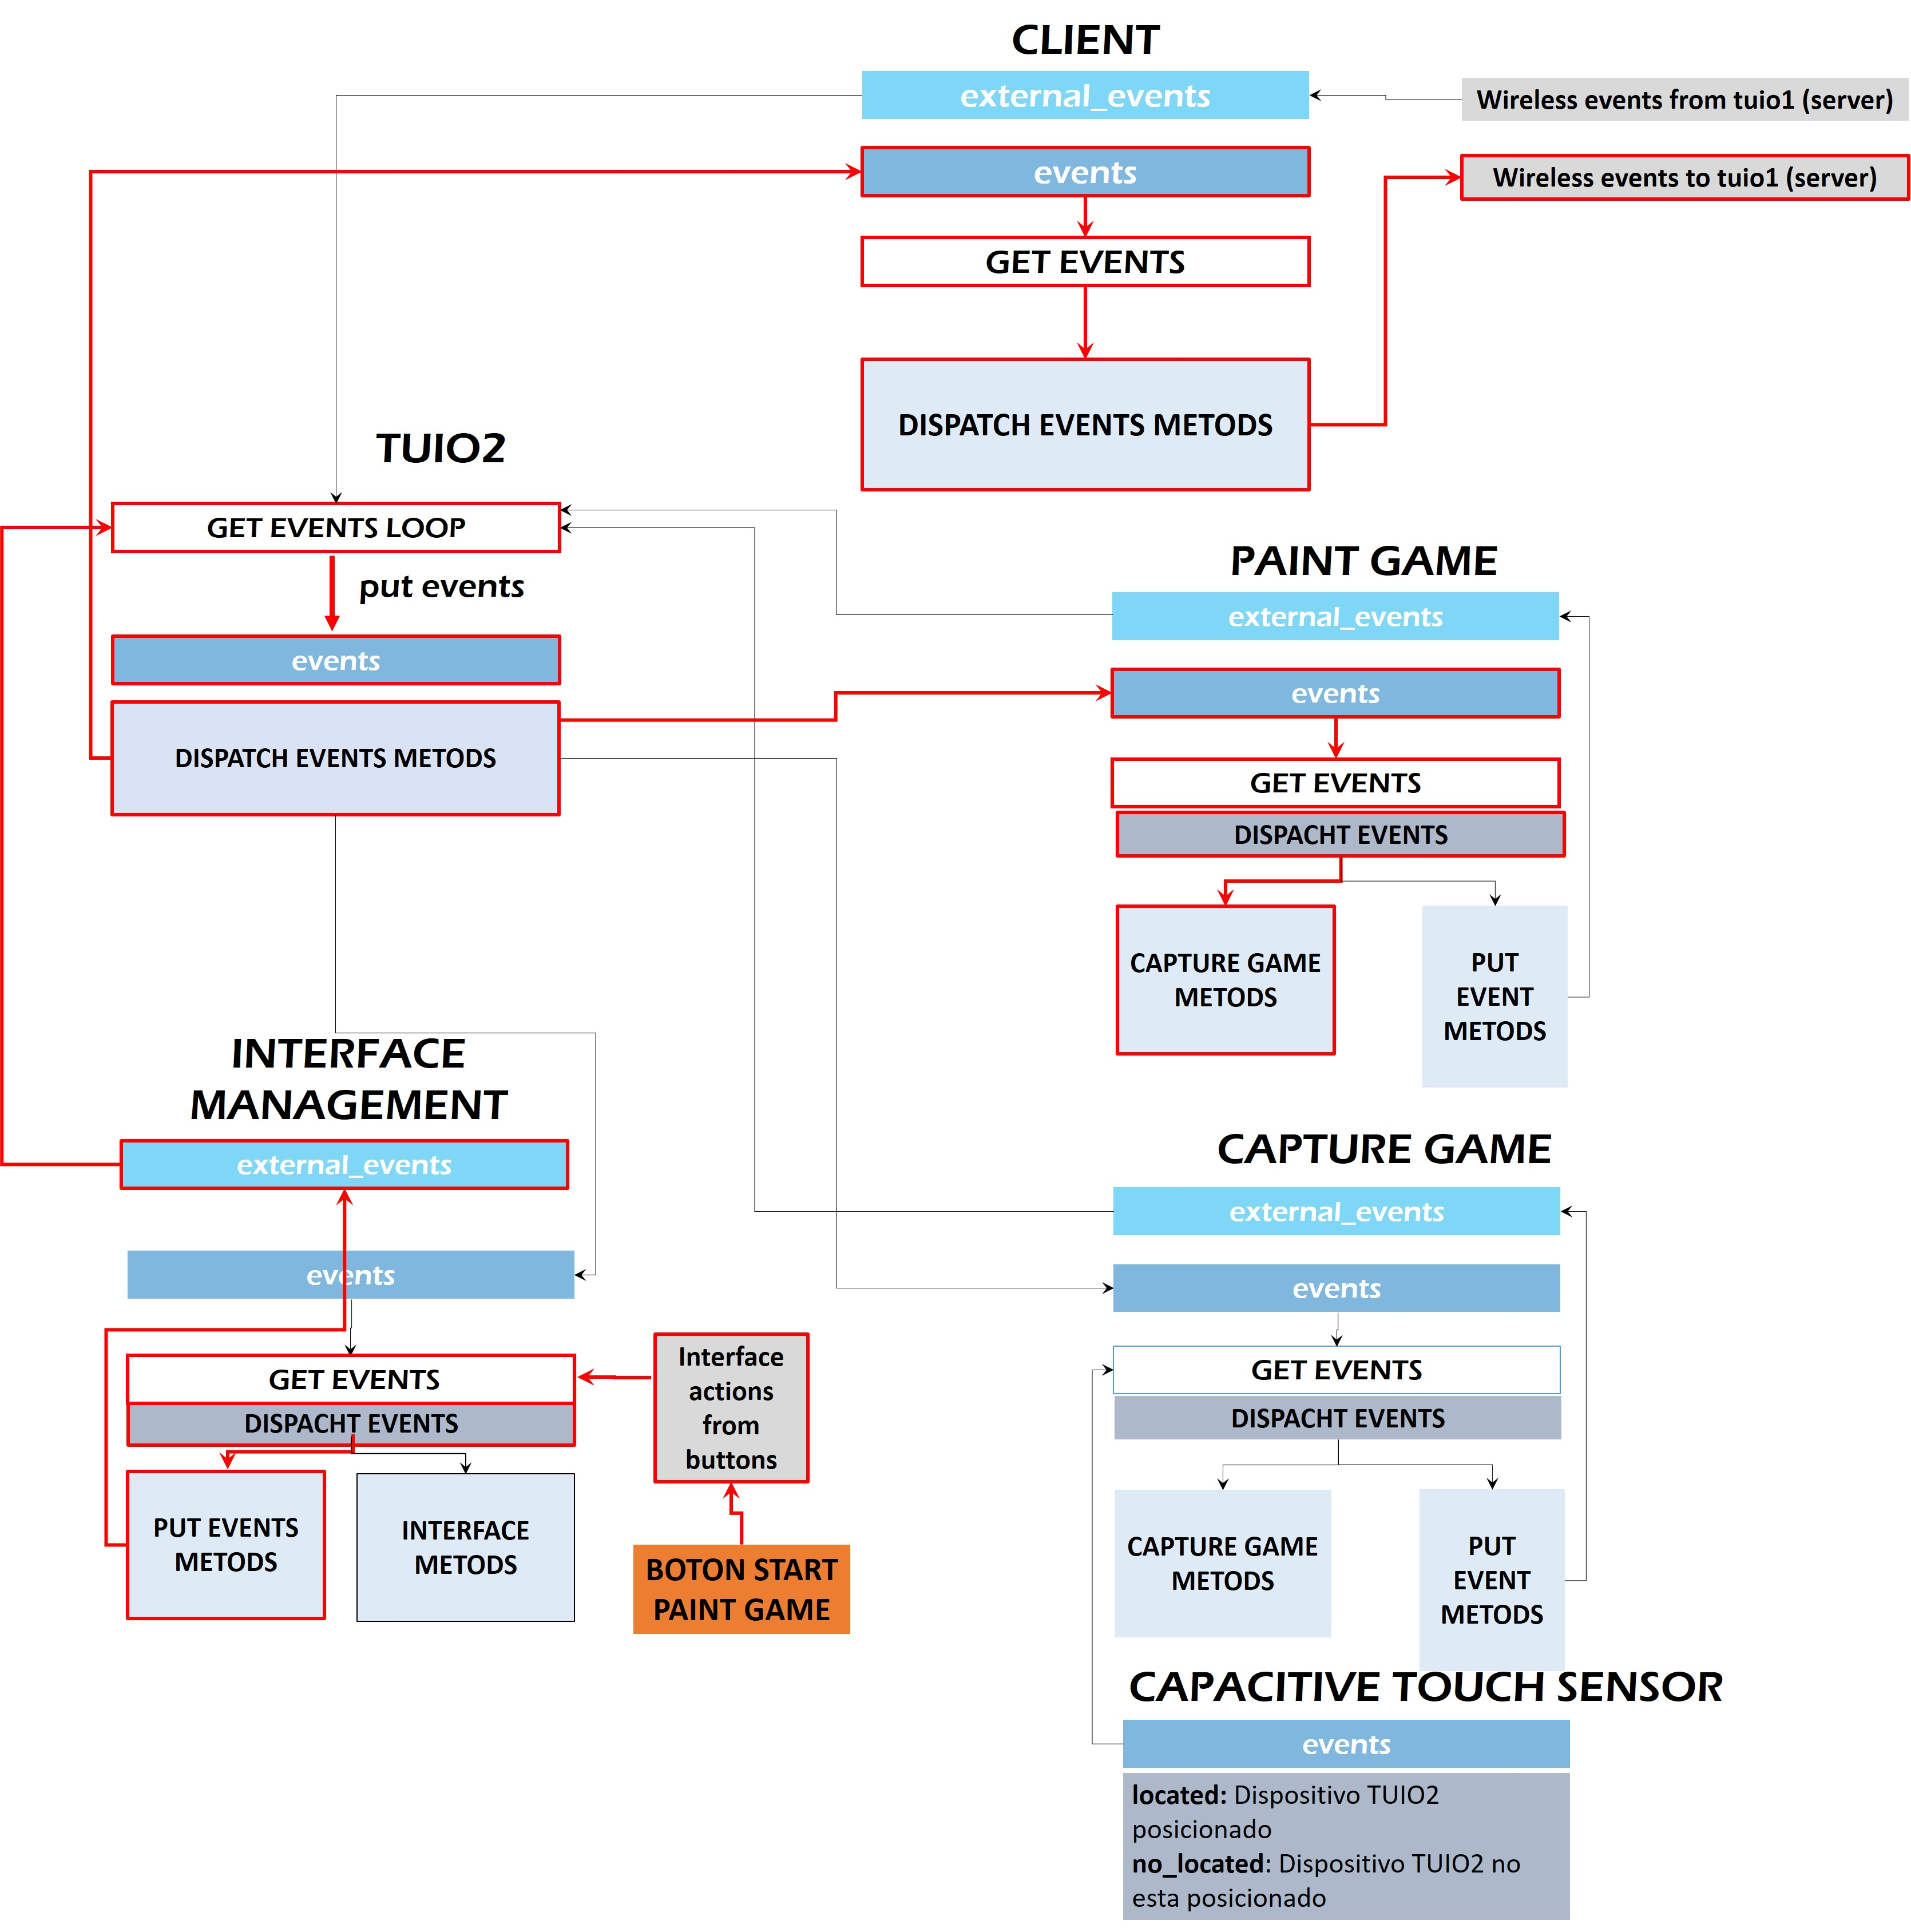
\includegraphics[width=0.9\textwidth]{events_tuio2.jpg}
\caption{Manejo de eventos en \emph{TUIO2}. Pruebas comenzar juego \textbf{PAINT GAME}.}
\label{fig:eventosTUIO2}
\end{center}
\end{figure}

\begin{figure}[!h]
\begin{center}
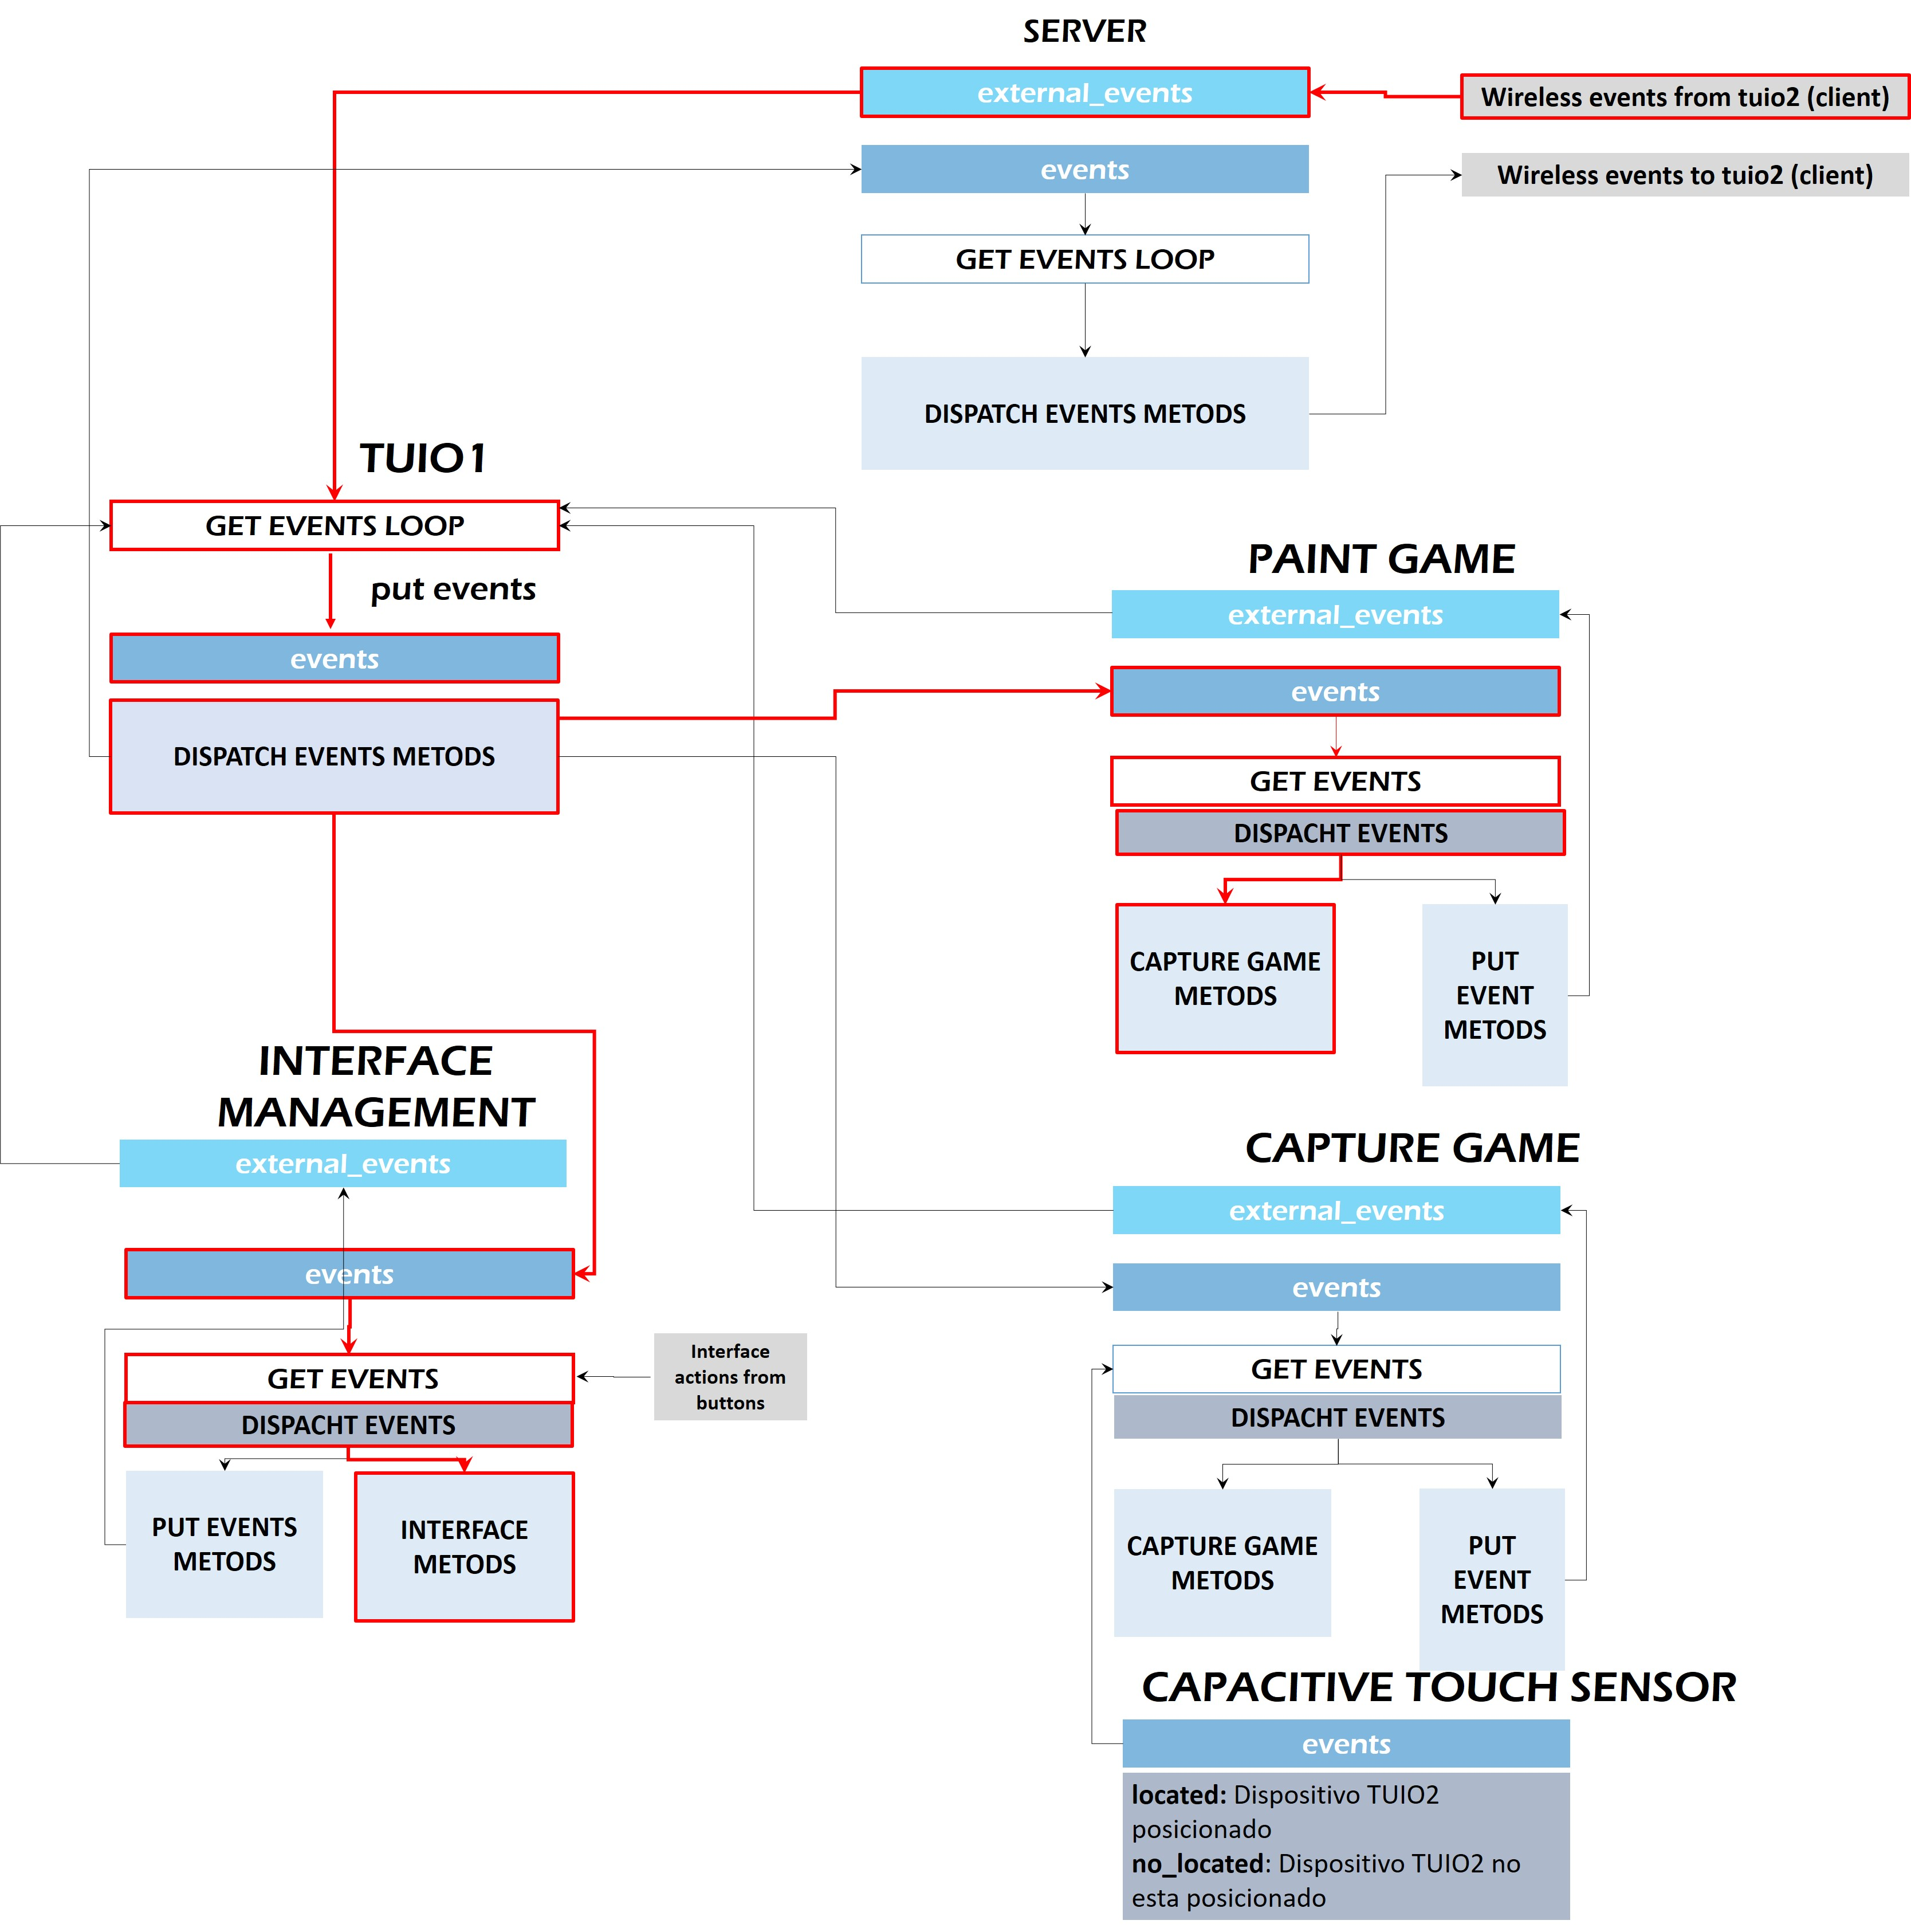
\includegraphics[width=0.9\textwidth]{events_tuio1.jpg}
\caption{Manejo de eventos en \emph{TUIO1}. Pruebas comenzar juego \textbf{PAINT GAME}.}
\label{fig:eventosTUIO1}
\end{center}
\end{figure}

\section{Diseño software de la interfaz gráfica.}



\section{Actualización software de la aplicación.}




